\chapter[]{I fazzoletti per istruzione militare in Italia}
\graphicspath{ {./images/chapter3/} }

Il testo è stato ricavato dagli articoli di Dirk  Ziesing e da alcune scritte e significativi particolari dei singoli manufatti. 



De Angeli-Frua
   La stamperia italiana per i fazzoletti da istruzione è nata a Saronno, cittadina a nord di Milano,  fondata da Ernesto De Angeli (1849-1907). Egli acquisì la propria formazione professionale grazie al barone Costanzo Cantoni, fondatore dell’industria tessile in Italia. La sua azienda di filatura e tessitura del cotone (cotonificio) nasceva a Castellanza già dal 1845. Nel 1872 venne fondata la “Società Ernesto De Angeli \& C” e nel 1878 denominata “Stamperia milanese per stoffe Cantoni”. De Angeli conquistò una grande reputazione nella sua città natale e nel 1895 venne nominato senatore.
   In questa situazione si deve però citare anche Giuseppe Frua (1855-1937) che, già dall’età di 16 anni, cominciò a conoscere il lavoro della tessitura presso un’azienda tedesca. Al suo rientro in Italia, dapprima trovò un’occupazione nell’azienda tessile Caprotti quindi, nel 1875, entrò a servizio di Eugenio Cantoni, figlio e successore del già nominato Barone. Nel 1879 l’attività Frua venne spostata nella sede di Castellanza. Nel 1883 egli sposò Anna De Angeli e nello stesso tempo divenne procuratore dell’azienda del cognato. Dopodiché, nel 1890 divenne partner della fabbrica tessile dei fratelli Banfi di Legnano (Anonima Frua \& Banfi) e nel 1896 si associano Ernesto De Angeli e Giuseppe Frua concentrando filatura, tessitura e stampa in un’unica azienda, denominata “De Angli-Frua”.
   All’inizio del ventesimo secolo (1900) si sperimentò  anche  la  
produzione  in  proprio  della  seta. A tale scopo    venne acquisto un terreno sul lago di Orta adattando la precedente piantagione di viti e alberi da frutta in gelsi, le cui foglie erano essenziali per l’allevamento dei bruchi. Nello stesso periodo venne inoltre acquistato un sontuoso edificio del 18° secolo sul lago Maggiore, come sede di rappresentanza. Questa villa De Angeli-Frua( a Laveno) – come gran parte degli edifici di origine aziendale a Milano e nei suoi dintorni – esiste ancora oggi.
   In definitiva, nel 1937 figuravano complessivamente cinque fabbriche con 11.000 dipendenti. La fabbrica di Gerenzano, vicino a Milano, divenne oggetto di modello, così come la residenza del direttore e i vicini edifici aziendali, cantine, scuole e un asilo aziendale. A seguito però dei problemi economici dell’industria tessile europea derivante dalla concorrenza asiatica, l’azienda chiuse le porte nel 1970..

Sguardo d’insieme
   La stamperia tessile milanese si dedicò tra l’altro anche ai fazzoletti militari d’istruzione. Per questo, attribuì particolare significato al materiale cartografico, e in seguito venne integrata negli schemi di numerazione italiani. Così nacque nel 1884 il primo fazzoletto con la stampa di una scena militare italiana. Seguirono fazzoletti orientati alla tecniche militari e alla fine vennero nuovamente rappresentati temi geografici.

Fazzoletto italiano n° 1   
La mappa sul fazzoletto in formato 64x58 cm mostra lo stivale italiano, le isole maggiori di Sardegna e Sicilia così come le isole restanti. Oltre alle strade di ordine (classe) 1, 2 e 3 e alle linee ferroviarie, figurano i numeri dei dodici corpi d’armata e le sedi dei comandi e delle fortezze. 
   Il titolo sovrimpresso recita “Carta dimostrativa delle circoscrizioni militari del regno d’Italia 1884”. Tutt’intorno sono rappresentati gli stemmi delle diverse aree d’amministrazione italiane (come dire: le provincie), con i numeri dei rispettivi  abitanti. Negli angoli e al centro  dei lati figurano gli stemmi delle città maggiori: Roma, Firenze, Napoli, Genova, Torino, Palermo, Milano e Venezia. Tra di essi appaiono invece, in ordine alfabetico e in senso orario, tutte le altre città da Alessandria a Vicenza. 


Fazzoletto italiano n° 2

   Il secondo fazzoletto della collezione italiana descrive il fucile della fanteria Modello 1870-87. Esso riporta al centro la scritta “Fucile Modello 1870-87” e sui margini le scritte “Fazzoletto militare N° 2 – (Privativa Industriale)” nonché “Stamperia E. De-Angeli \& C – Milano”. La spiegazione delle due date consiste nel fatto che nel 1887 venne modernizzato il precedente modello del 1870. Un fazzoletto di questa serie solo con il modello originale non venne alla luce,  anche  se  è  certo che esistesse e che venne stampato dalla società Rolffs dedita ai fazzoletti di istruzione austro-ungarici  (vedi fazzoletto 2A di pag.44 ).
   Con il loro aggiornamento, le precedenti armi vennero fornite con il corredo di un caricatore più ampio. Il caricatore con magazzino per quattro cartucce venne sviluppato per il capitano d’artiglieria Giuseppe Vitali. Sullo stesso principio vennero del resto realizzati un anno dopo anche i fucili olandesi Beaumont. Poiché le armi italiane vennero adeguate in grandi quantità,  è molto raro trovare i fucili Vetterli proprio in versione originale. Per la guida del caricatore, la sua carrozzeria riportava un’apertura nella parte inferiore. Per compensare l’indebolimento della struttura, nel legno del fucile venne integrato un piatto metallico. Oltre a ciò si integrò anche una barra per la guida della punta della pallottola, mentre il coperchio di protezione sull’apertura della cassa venne a sua volta rafforzata e compensata con un anello metallico. 
Infine seguirono anche una modifica della leva di sicurezza e l’irrobustimento della baionetta. Il mirino a quadrante già abbozzato da Vecci rappresentò anch’esso una modifica apportata sul Modello 1870 già nel 1881.

Fazzoletto italiano n° 3
  I fucili costruiti nel 1887 vennero modificati già pochi anni dopo attraverso un nuovo fucile a ripetizione. Anche per esso venne creato un nuovo fazzoletto d’istruzione. Esso venne intitolato “Fucile modello 1891”, con riporto sulla fascia    esterna    orizzontale   del   testo   “FAZZOLETTO MILITARE N°3 – (PRIVATIVA INDUSTRIALE), nonché “STAMPERIA E. DE-ANGELI \& C – MILANO”.    Il nuovo fucile italiano venne ufficialmente introdotto in data 29 marzo 1892. Esso è a struttura di caricatore basato sul principio di Mannlicher. Ferdinando von Mannlicher ne ricavò una licenza brevettuale di 300.000 lire. Il sistema di otturazione venne progettato nell’arsenale cittadino dei fucili di Torino sotto la direzione di Salvatore Carcano (1827-1903) e in collaborazione con comandanti e ingegneri militari. In tale circostanza viene talvolta fatto anche il nome di Gustavo Parravicino, Presidente della Commissione per l’approvazione dei nuovi fucili.   Dalla solida costruzione, quest’arma aveva una capacità di magazzino di sei cartucce. Il calibro relativamente piccolo di 6,5x52 mm determinò subito il vantaggio che un singolo soldato poteva portare con sé un consistente quantitativo di munizioni. D’altro lato la sua criticità generalmente riconosciuta consisteva in operazioni di limitata portata balistica. Anche perciò, le cartucce Carcano riportavano il proiettile con la punta arrotondata, ancor oggi usata, e come già da tempo anche altre nazioni avevano fatto con la punta dei loro proiettili.  
   Un ulteriore svantaggio proveniva dalla lunghezza del successivo modello realizzato per la fanteria. Esso riporta un mirino scorrevole con un gittata da 450 a 2000 metri. La misura di 1,60 m dal calcio all’innesto della baionetta derivava dal principio che, negli scontri con la cavalleria, un fante potesse attaccare in modo efficace anche un cavaliere a cavallo. Per la guerra di trincea, che si svilupperà durante la prima guerra mondiale, questa lunghezza sarà invece di forte intralcio. 
  Perciò nella famiglia dei fucili Carcano comparvero delle successive versioni accorciate. Il “Moschetto Cavalleria” venne sviluppato per la Cavalleria nel 1893 e più tardi trasformato anche in fucile da caccia. 
   Tra le altre cose, è interessante la molteplicità delle varianti delle cartucce, sempre stampate sul Fazzoletto Carcano, e riportate nella sua parte bassa.  Accanto alle normali cartucce sottili e pallottole con copertura in nichel (“A pallottola”), c’erano quelle “da esercitazione”, quella “a salve” e le munizioni per tiro a segno. Una particolarità consiste nelle pallottole a sparo singolo e in quelle a mitraglia.
Fazzoletto cartografico italiano del 1912
   L’aspetto del fazzoletto cartografico del 1912 riporta il medesimo titolo della prima stampa del 1884 ed è identico anche il formato di 64x58 cm. La cornice degli stemmi rimane in sostanza la medesima, con le seguenti modifiche: al posto di Porto-Maurizio subentra Imperia, dato che era stata assorbita nella medesima zona rivierasca unitamente alla vicina Oneglia. Rovigo viene collocata dopo Reggio Calabria e Reggio Emilia, adesso in corretto ordine alfabetico. Inoltre, l’area sopra il titolo viene riempita con cinque ulteriori stemmi. A quanto pare infatti erano state semplicemente dimenticate le circoscrizioni di Campobasso, Grosseto, Lecce, Potenza e Siracusa.
   A ciascuna circoscrizione viene inoltre associato il numero dei residenti. Così, per esempio per Roma, figura l’indicazione di 864.851 abitanti.  Viene  inoltre  riportato  il numero complessivo degli italiani nel 1912, per un valore di 34.978.634 unità con una densità di 268.682 persone a kmq.
   È anche presente un essenziale completamento alla carta geografica con il riporto delle colonie possedute dall’Italia alla fine del 19° secolo. Due dettagliate carte geografiche riportano il sovra titolo “POSSESSIONI D’OLTRE MARE COLONIA ERITREA – SOMALIA - TRIPOLITANIA” (possedimenti d’oltre mare). Sul Mar Rosso era stata acquisita la colonia italiana d’Eritrea nel 1890. Dopo la seconda guerra mondiale questo territorio costituì una federazione con gli Etiopi. Solo dopo una guerra di una decina d’anni l’Eritrea divenne uno stato indipendente.   Sul Corno d’Africa, al di sotto del Golfo di Aden, si trovava la colonia “Somalia Italiana”.  
Fazzoletto cartografico italiano del 1918
   Alla fine della prima guerra mondiale venne prodotto un altro fazzoletto cartografico italiano, con titolo “ITALIA – REDENTA E UNA PER VALORE DEI SUOI SOLDATI – 3 NOVEMBRE 1918”. Il 3 novembre 1918 segnò attraverso la firma dell’armistizio tra l’Italia e l’Austria-Ungheria la fine della prima guerra mondiale su questo fronte.
   Questa Carta riporta lungo la cornice la scritta “STAMPERIA ITALIANA DE ANGELI MILANO – BREVETTATO”. Questo fazzoletto con lati di circa 52x52 cm è leggermente più piccolo del suo predecessore. Le aree coloniali  non  sono  più  rappresentate, ma in cambio seguì un allargamento nel NORD attraverso i territori de Sud Tirolo e del’Istria sottratti all’Austria-Ungheria.  
   Parimenti aumentò il numero degli stendardi di cornice, che venne organizzato in una nuova fila disposta nell’area inferiore del fazzoletto. Essa comprende le nuove circoscrizioni e sedi di Ala, Arco, Bolzano, Capodistria, Gorizia, Istria (con un errore di stampa), Levico, Pola, Fiume, Parenzo, Pisino, Riva, Rovigo, Rovereto, Volosca e Zara. Nel fazzoletto del 1918 si soprassedette al riporto del numero degli abitanti e delle strutture militari. 

\newpage

Nota esplicativa  
   Del fazzoletto sulla cavalleria (vedi pag. 52) l’unica cosa certa è che il prodotto è della stamperia E. De Angeli. Attualmente non siamo in grado di riportare altre documentazioni e/o spiegazioni. La stessa cosa vale per il manufatto sulle armi pesanti che viene effigiato a pagina 53. Questi due fazzoletti però documentano che oltre ai fazzoletti cartografici venivano stampati anche quelli dedicati a reparti militari specifici.
   
\begin{figure}[h]
	\centering
		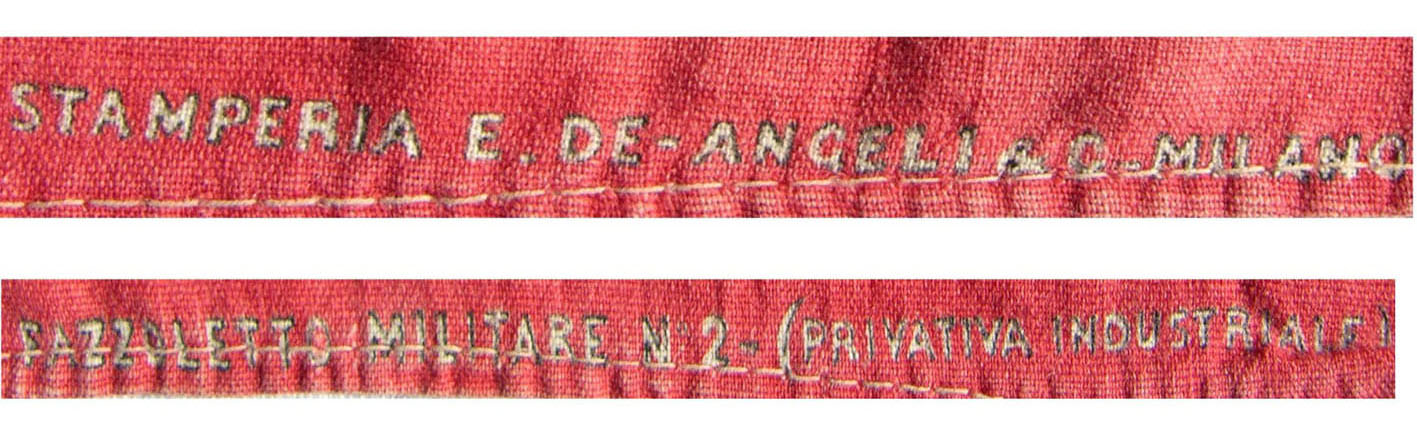
\includegraphics[width=\textwidth]{fazzoletto2_particolare.jpg}
	\caption{Particolare fazzoletto militare italiano n° 2. Certificazione della produzione stampata sul bordo inferiore.}
	\label{fig:fazzoletto2_particolare}
\end{figure}

\newpage

\begin{figure}[h]
	\centering
		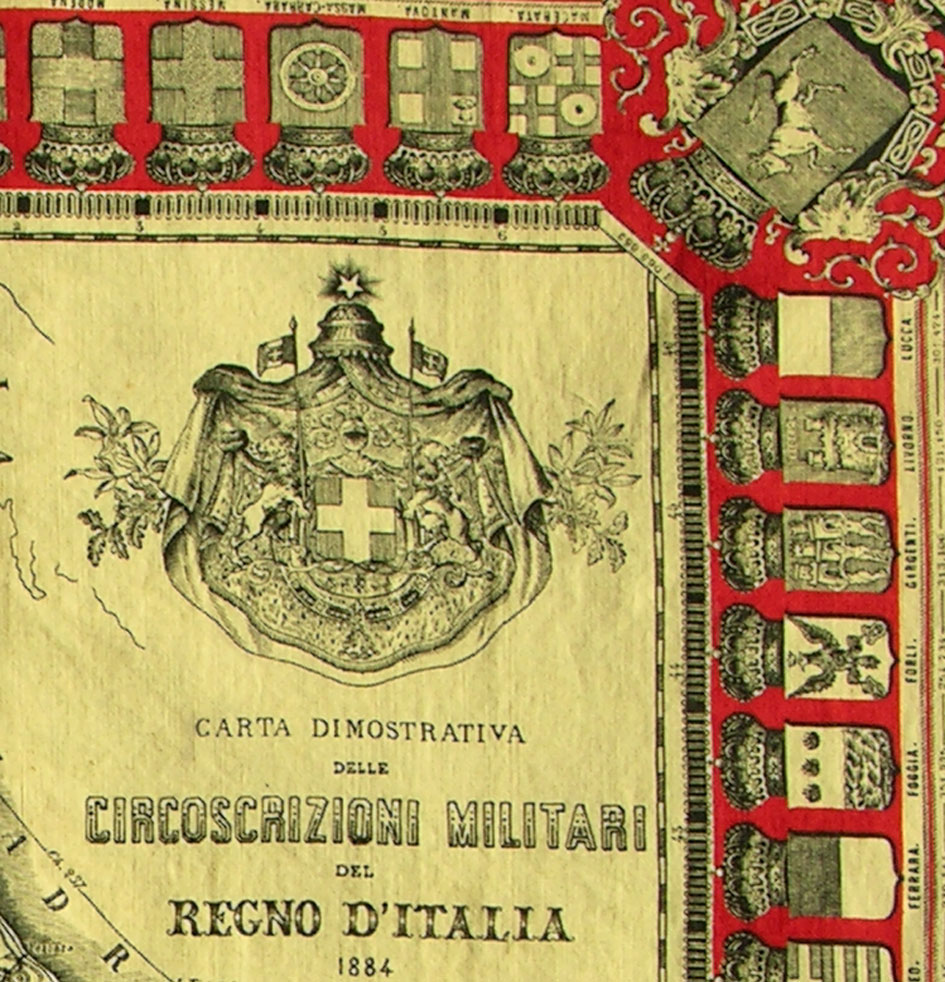
\includegraphics[width=\textwidth]{fazzoletto1_particolare.jpg}
	\caption{Particolare del fazzoletto militare n° 1}
	\label{fig:fazzoletto1_particolare}
\end{figure}

\newpage

\begin{figure}[h]
	\centering
		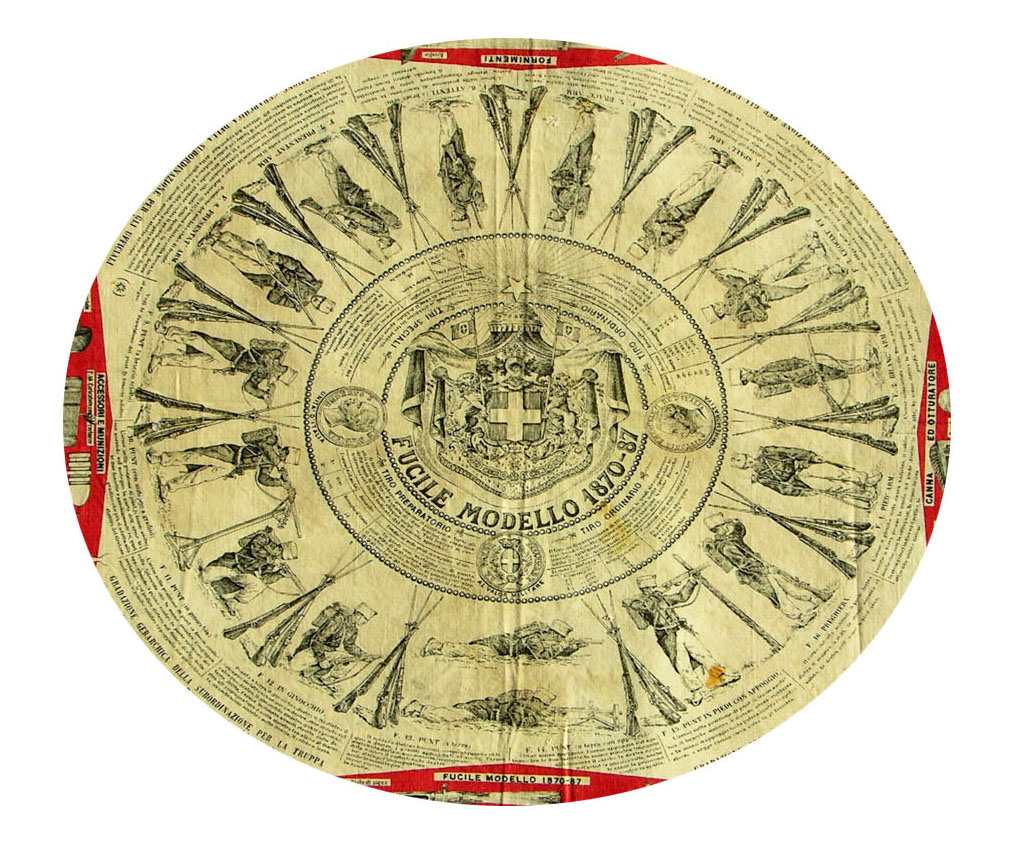
\includegraphics[width=\textwidth]{fazzoletto2_particolare_2.jpg}
	\caption{Particolare del fazzoletto  militare n° 2}
	\label{fig:fazzoletto2_particolare_2}
\end{figure}

\newpage

\begin{figure}[h]
	\centering
		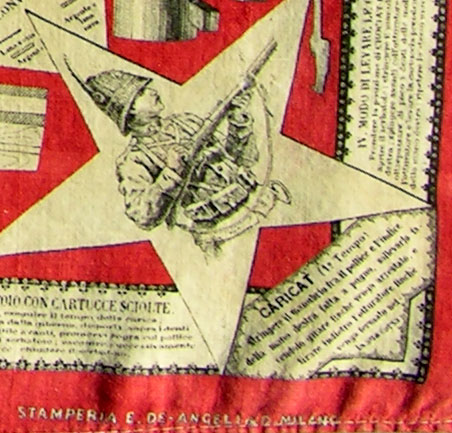
\includegraphics[width=\textwidth]{fazzoletto2_particolare_3.jpg}
	\centering
		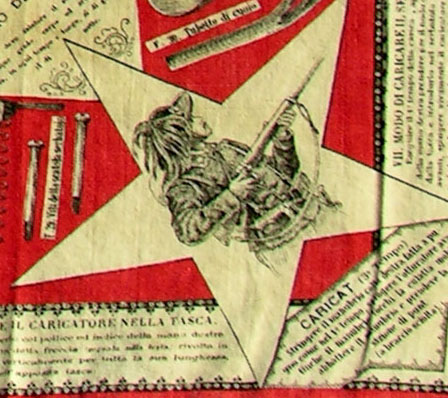
\includegraphics[width=\textwidth]{fazzoletto2_particolare_4.jpg}
	\caption{Particolari del fazzoletto militare n° 2. È evidente il nome del produttore nel bordo inferiore del modello in alto}
	\label{fig:fazzoletto2_particolare_3_4}
\end{figure}

\newpage

\begin{figure}[h]
	\centering
		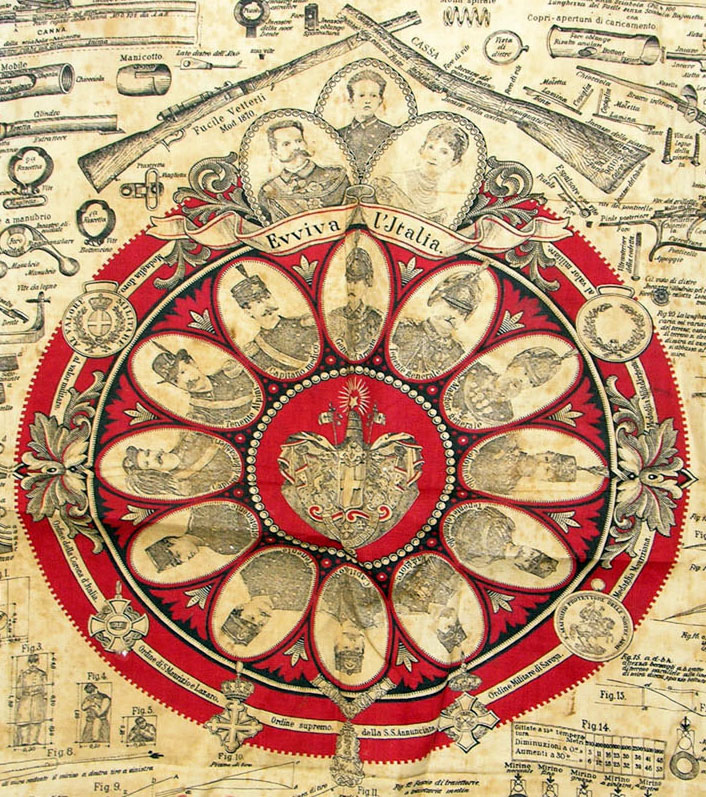
\includegraphics[width=\textwidth]{fazzoletto2A_particolare.jpg}
	\caption{Particolare del fazzoletto militare n°2°A.}
	\label{fig:fazzoletto2A_particolare}
\end{figure}

\newpage

\begin{figure}[h]
	\centering
		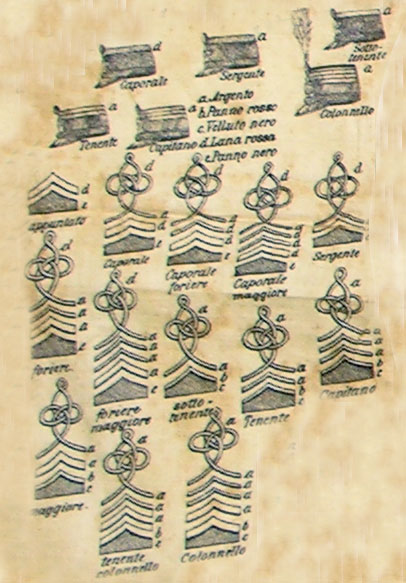
\includegraphics[width=\textwidth]{fazzoletto2A_particolare_2.jpg}
	\caption{}
	\label{fig:fazzoletto2A_particolare_2}
\end{figure}

\newpage

Altri particolari del fazzoletto militare  n° 2A

\begin{figure}[h]
	\centering
		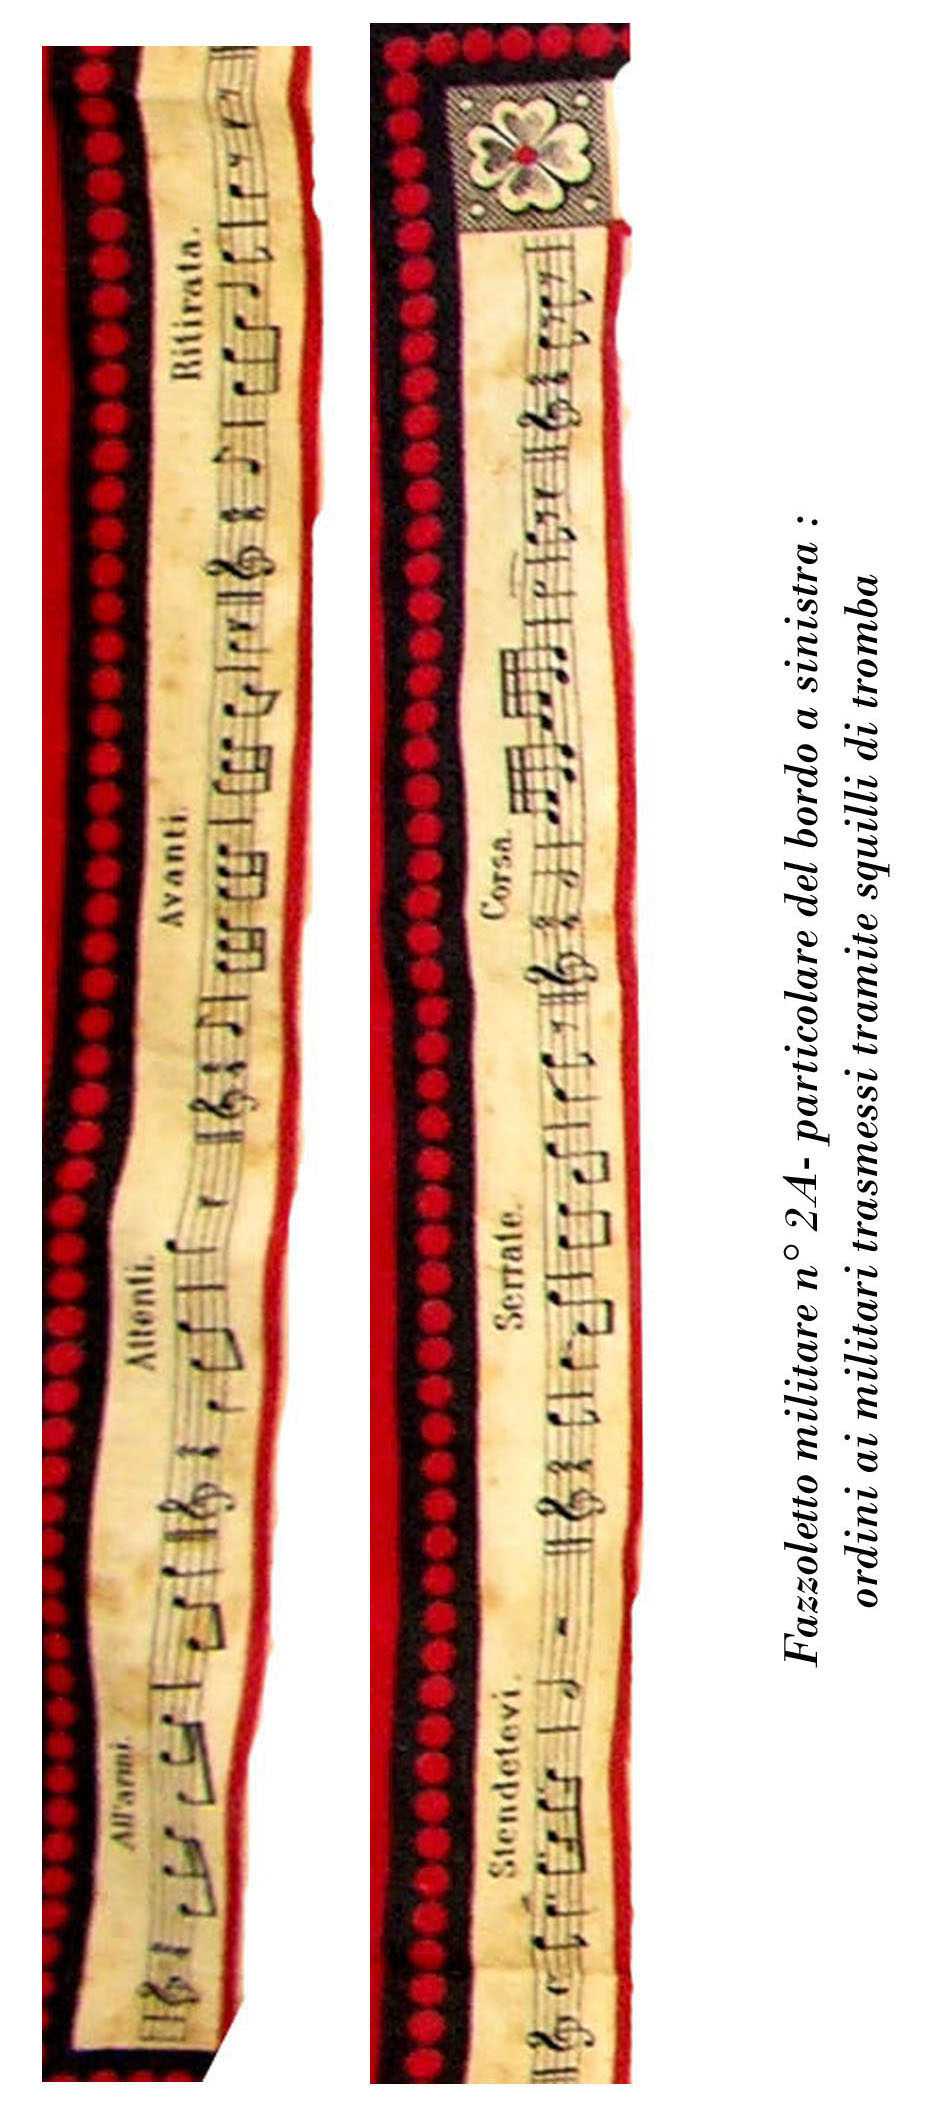
\includegraphics[width=\textwidth]{fazzoletto2A_particolare_3.jpg}
	\caption{}
	\label{fig:fazzoletto2A_particolare_3}
\end{figure}

\newpage

\begin{figure}[h]
	\centering
		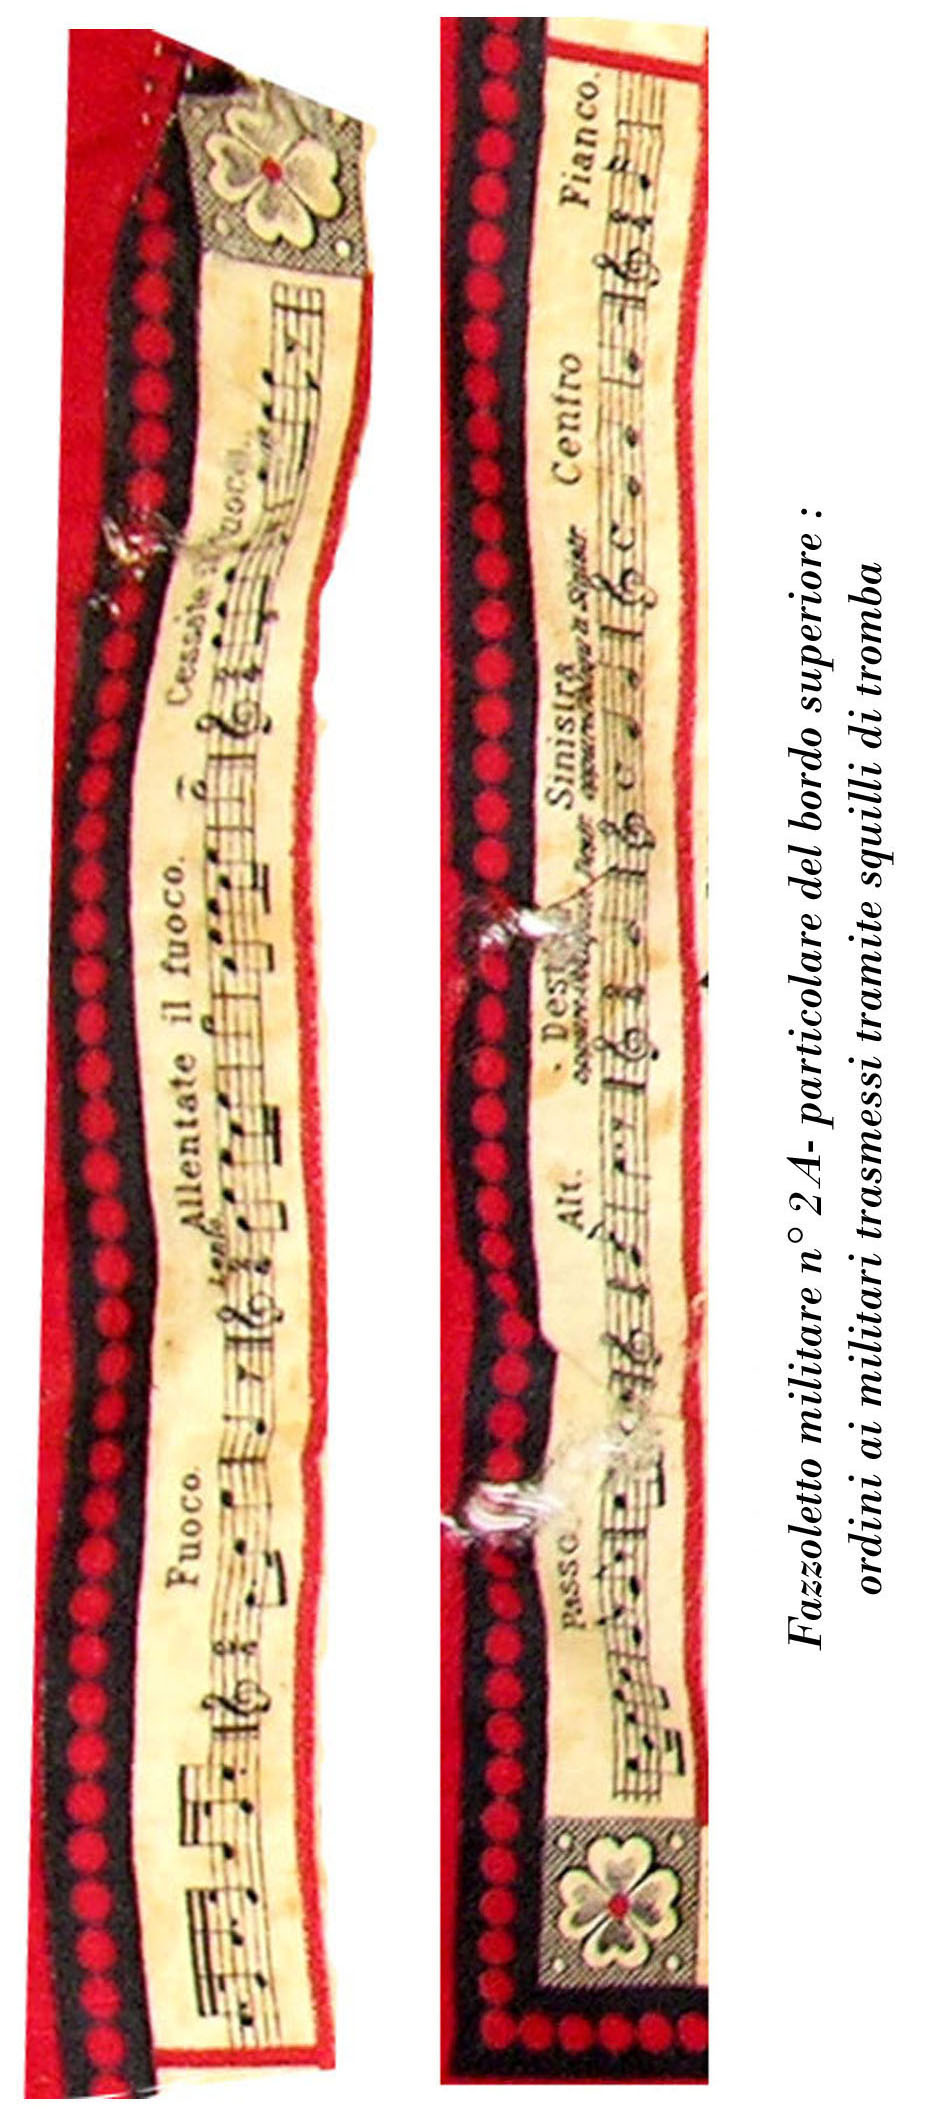
\includegraphics[width=\textwidth]{fazzoletto2A_particolare_4.jpg}
	\caption{}
	\label{fig:fazzoletto2A_particolare_4}
\end{figure}

\newpage

\begin{figure}[h]
	\centering
		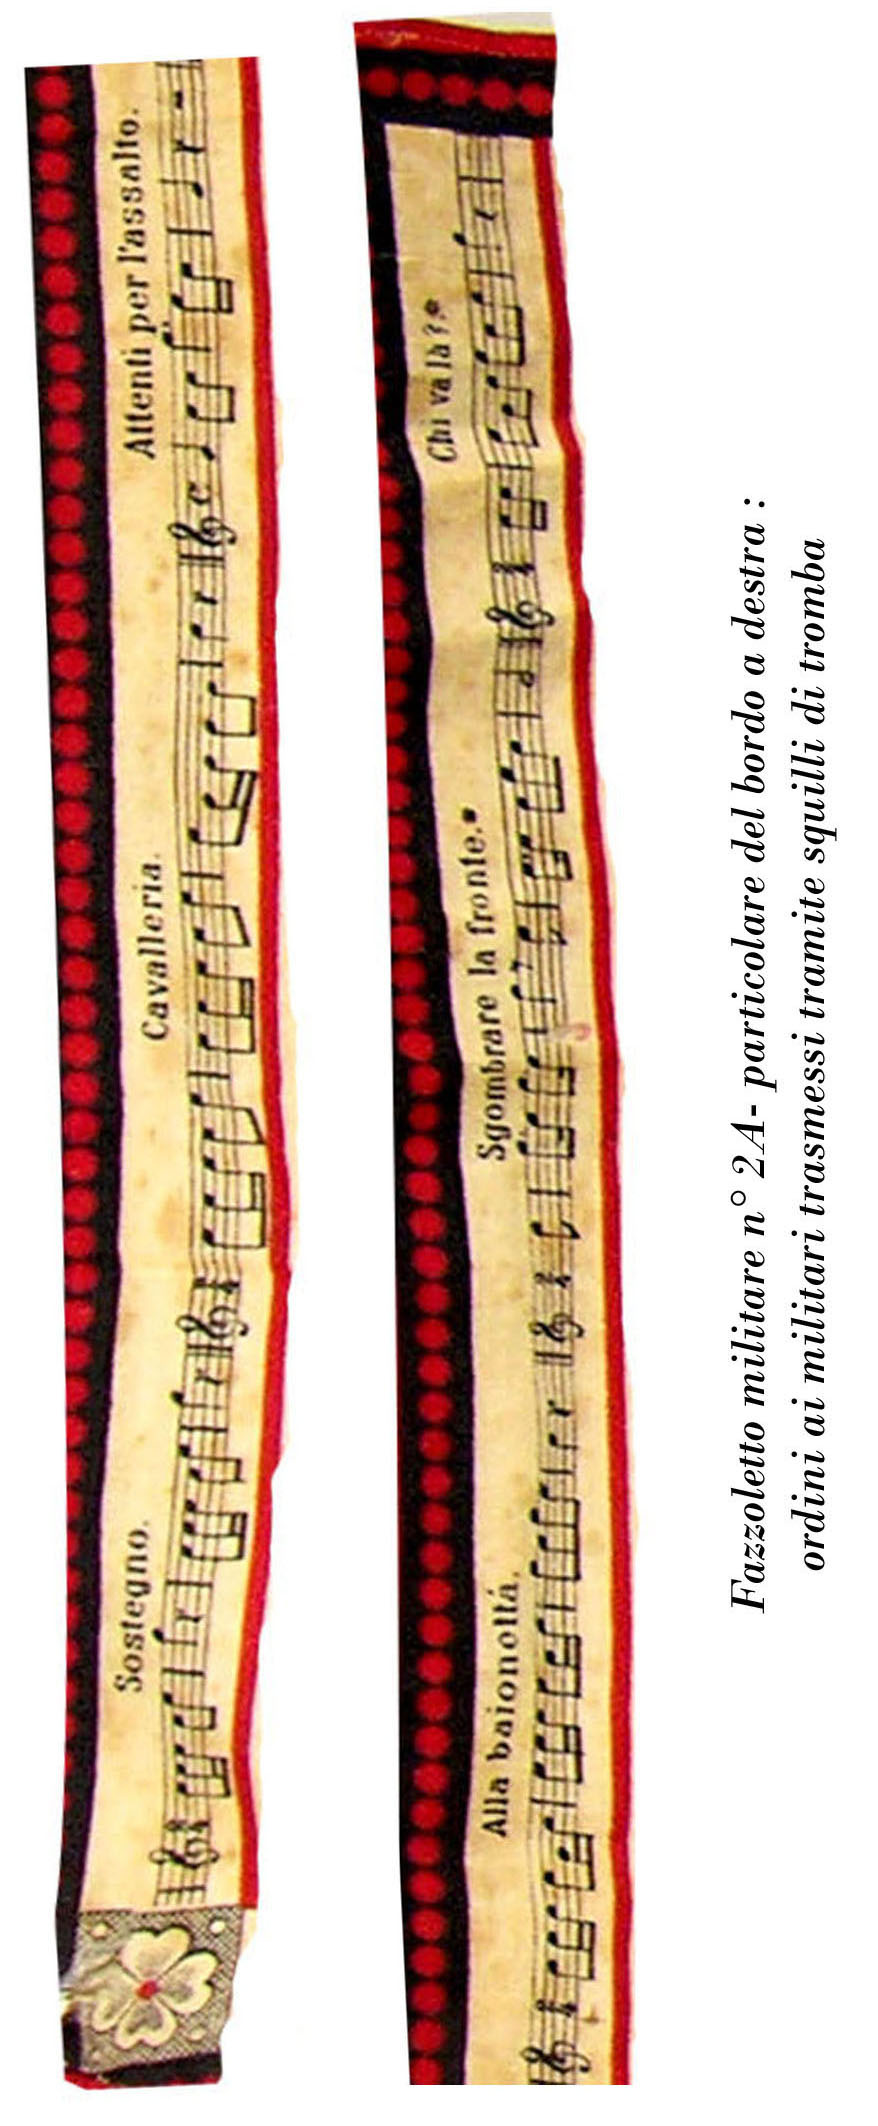
\includegraphics[width=\textwidth]{fazzoletto2A_particolare_5.jpg}
	\caption{}
	\label{fig:fazzoletto2A_particolare_5}
\end{figure}

\newpage

\begin{figure}[h]
	\centering
		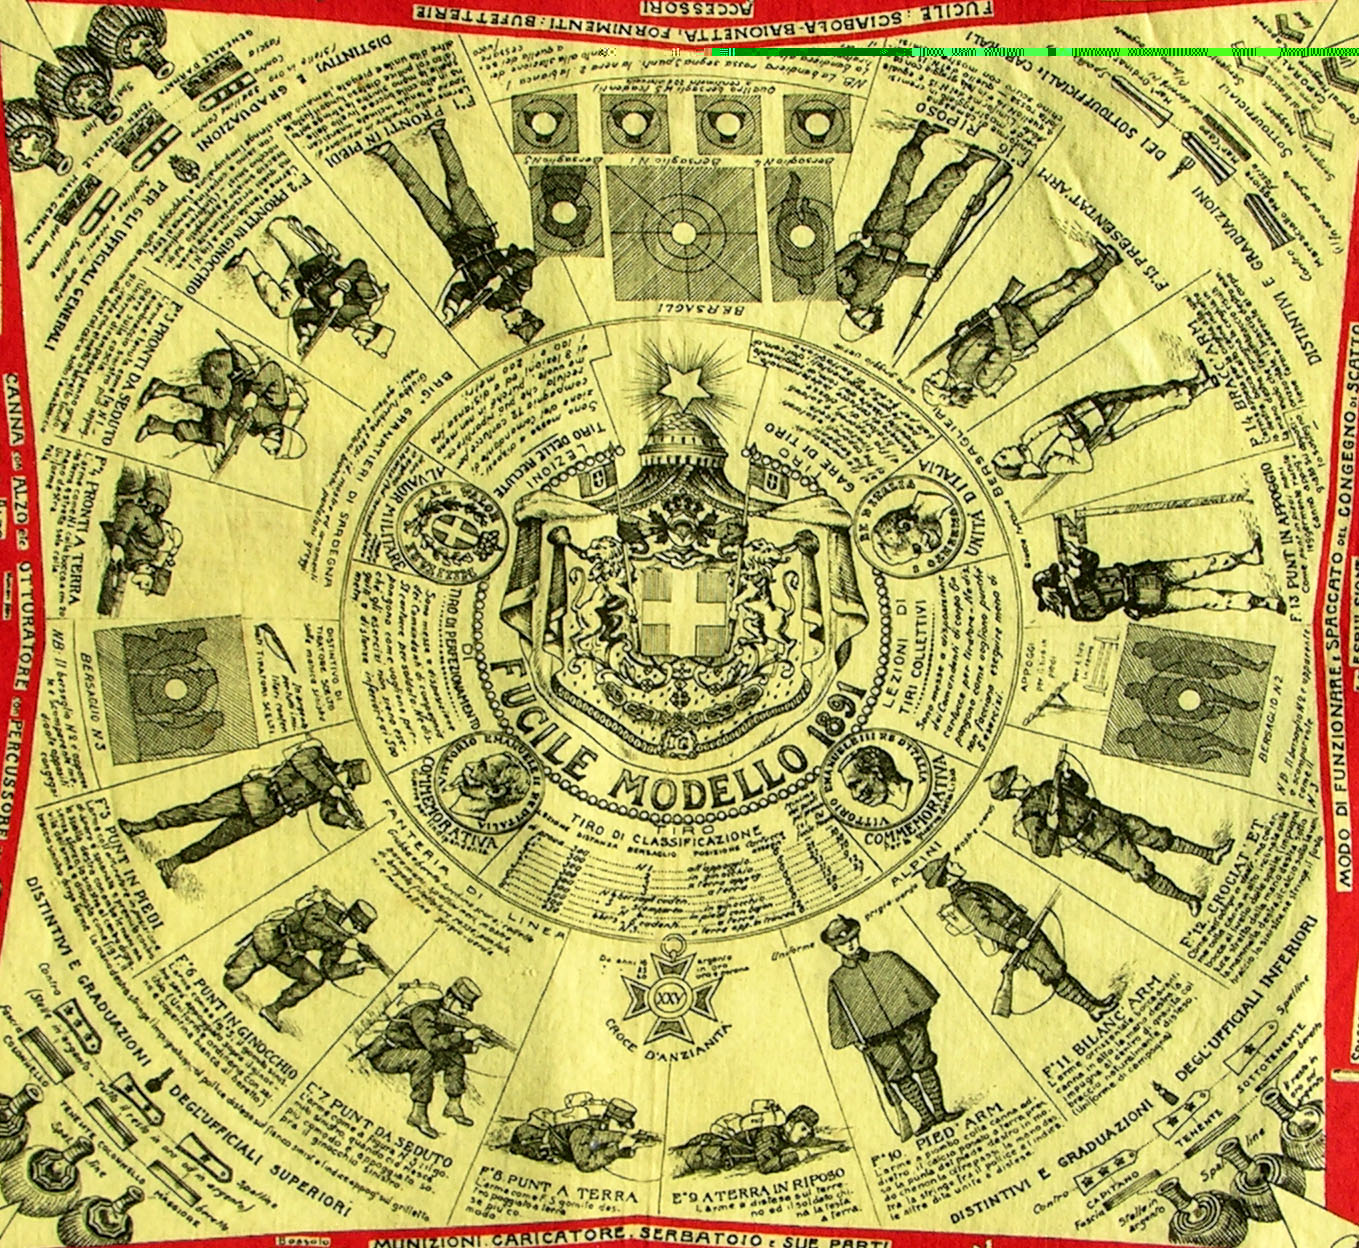
\includegraphics[width=\textwidth]{fazzoletto3_particolare.jpg}
	\caption{Particolare del fazzoletto militare n°3}
	\label{fig:fazzoletto3_particolare}
\end{figure}

\newpage

\begin{figure}[h]
	\centering
		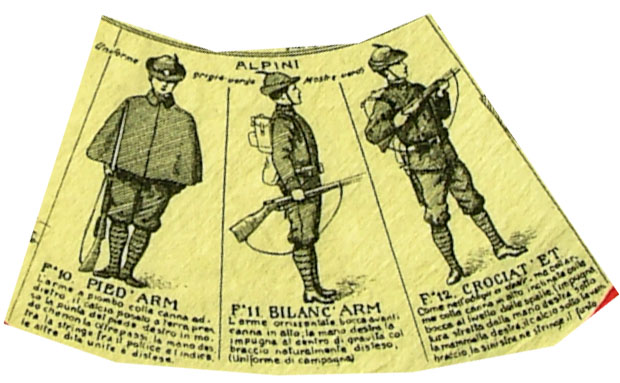
\includegraphics[width=\textwidth]{fazzoletto3_particolare_2.jpg}
	\centering
		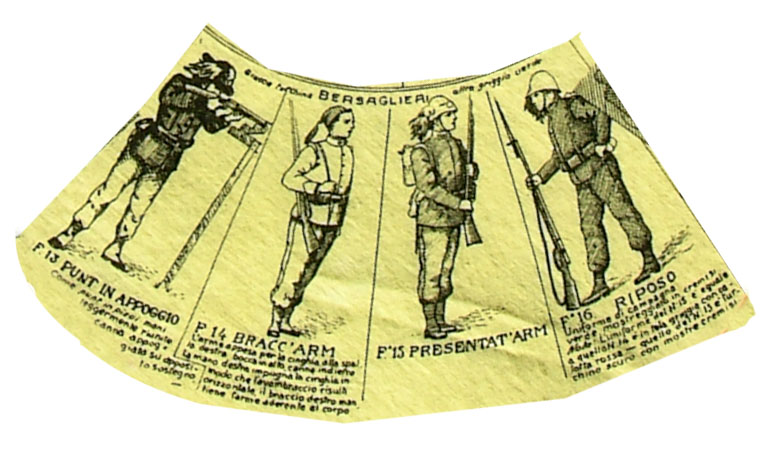
\includegraphics[width=\textwidth]{fazzoletto3_particolare_3.jpg}
	\caption{Altri particolari del fazzoletto militare n° 3}
	\label{fig:fazzoletto3_particolare_2_3}
\end{figure}

\newpage

\begin{figure}[h]
	\centering
		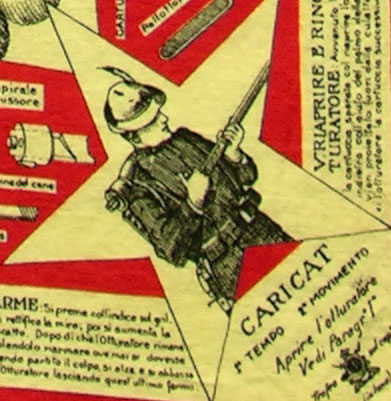
\includegraphics[width=\textwidth]{fazzoletto3_particolare_4.jpg}
	\centering
		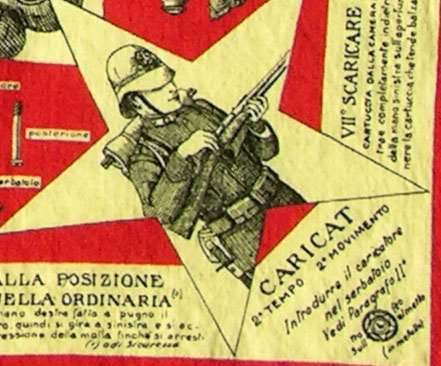
\includegraphics[width=\textwidth]{fazzoletto3_particolare_5.jpg}
	\caption{Altri particolari del fazzoletto militare n° 3}
	\label{fig:fazzoletto3_particolare_4_5}
\end{figure}

\newpage

\begin{figure}[h]
	\centering
		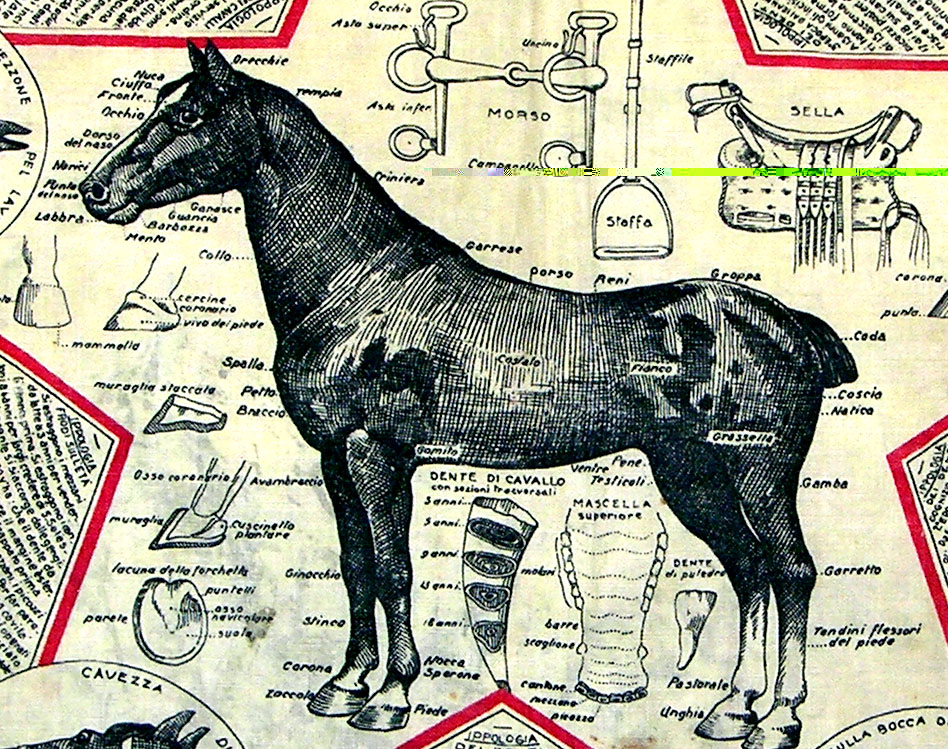
\includegraphics[width=\textwidth]{fazzoletto4_particolare.jpg}
	\caption{Particolare del fazzoletto militare n°4}
	\label{fig:fazzoletto4_particolare}
\end{figure}

\newpage

\begin{figure}[h]
	\centering
		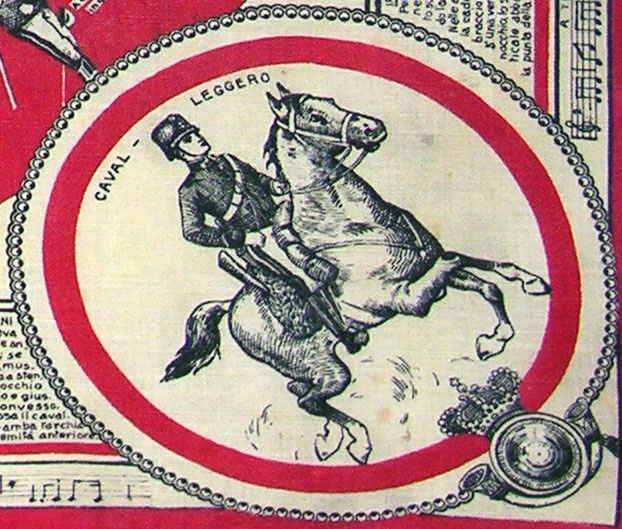
\includegraphics[width=\textwidth]{fazzoletto4_particolare_2.jpg}
	\centering
		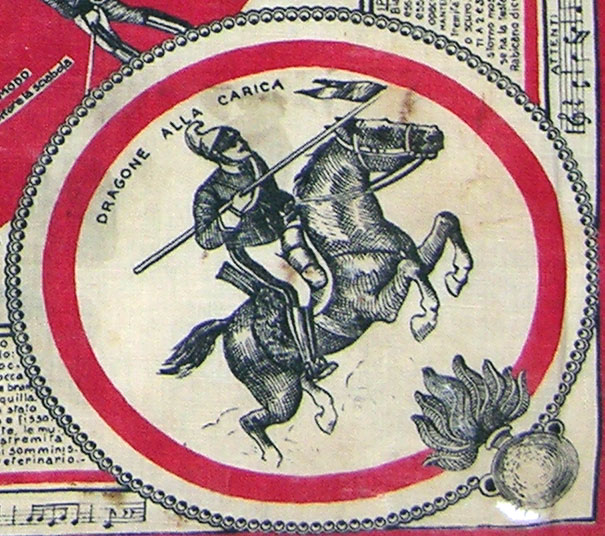
\includegraphics[width=\textwidth]{fazzoletto4_particolare_3.jpg}
	\caption{Particolari del fazzoletto militare n° 4}
	\label{fig:fazzoletto4_particolare_2_3}
\end{figure}

\newpage

\begin{figure}[h]
	\centering
		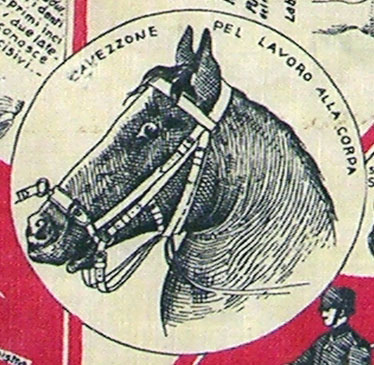
\includegraphics[width=\textwidth]{fazzoletto4_particolare_4.jpg}
	\centering
		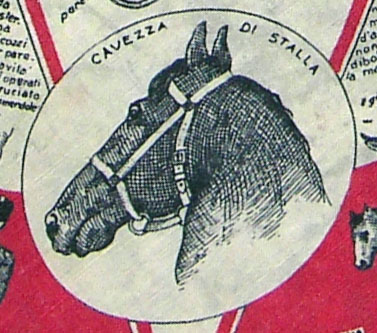
\includegraphics[width=\textwidth]{fazzoletto4_particolare_5.jpg}
	\caption{Dettagli d’immagini del fazzoletto militare n° 4}
	\label{fig:fazzoletto4_particolare_4_5}
\end{figure}

\newpage

\begin{figure}[h]
	\centering
		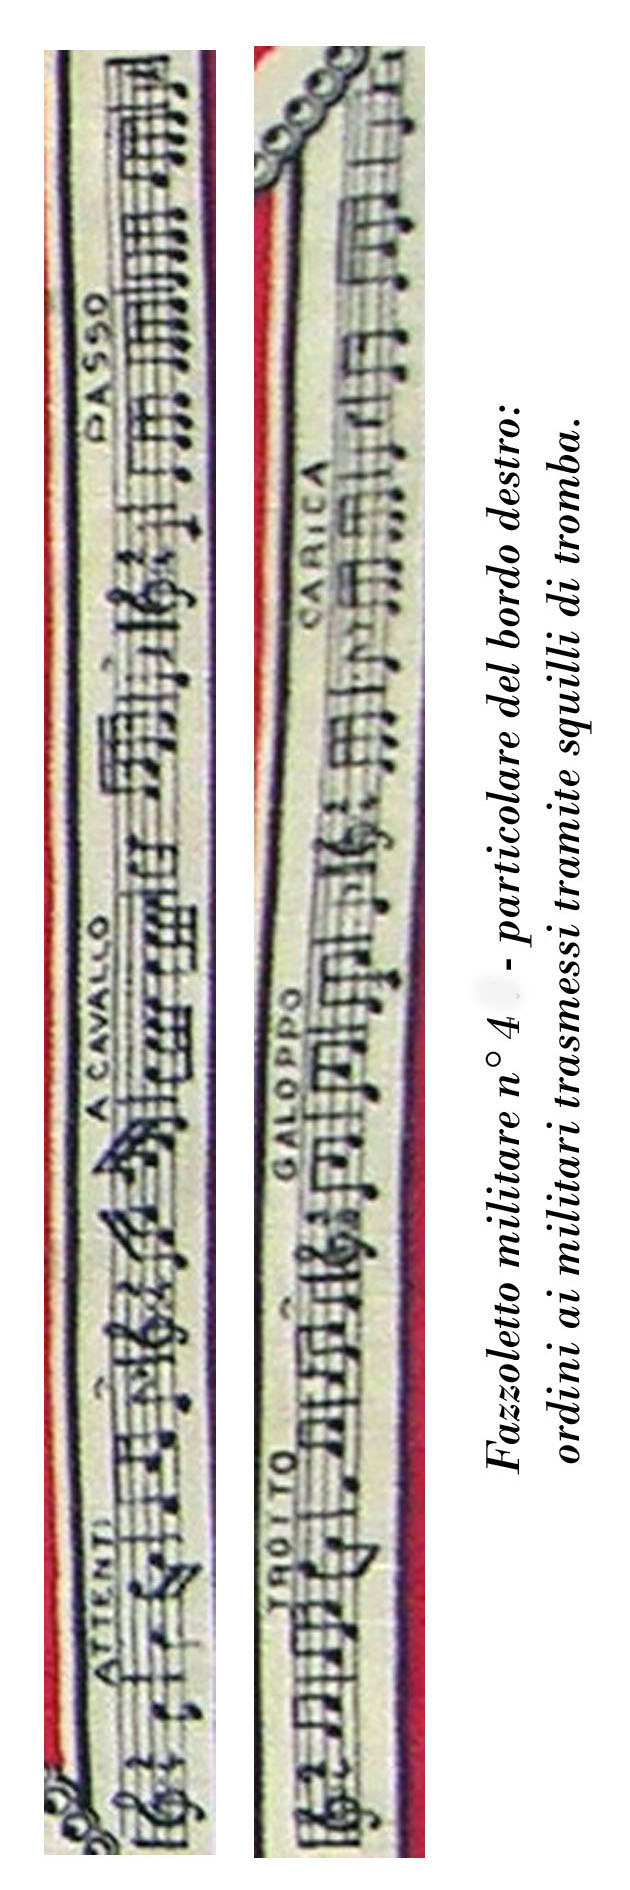
\includegraphics[width=\textwidth]{fazzoletto4_particolare_6.jpg}
	\caption{}
	\label{fig:fazzoletto4_particolare_6}
\end{figure}

\newpage

\begin{figure}[h]
	\centering
		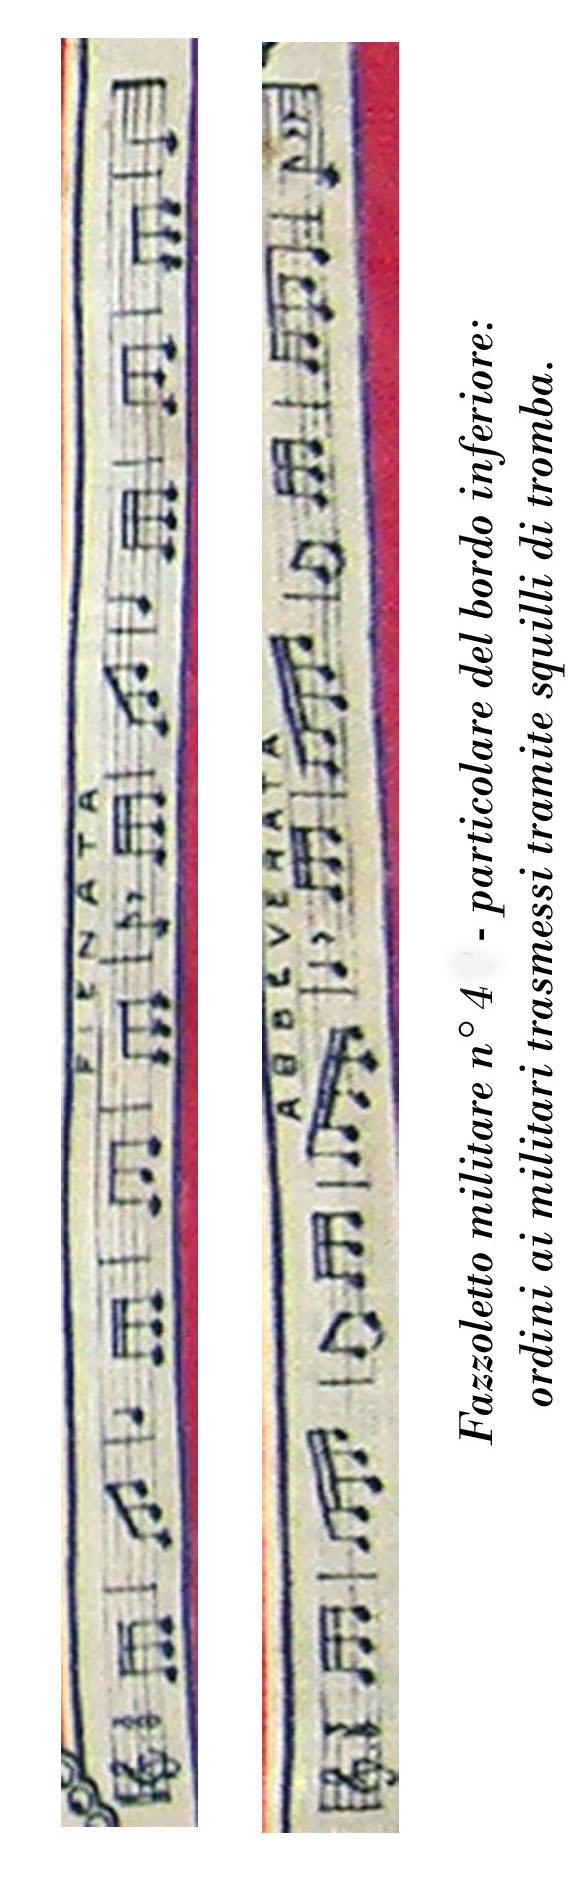
\includegraphics[width=\textwidth]{fazzoletto4_particolare_7.jpg}
	\caption{}
	\label{fig:fazzoletto4_particolare_7}
\end{figure}

\newpage

\begin{figure}[h]
	\centering
		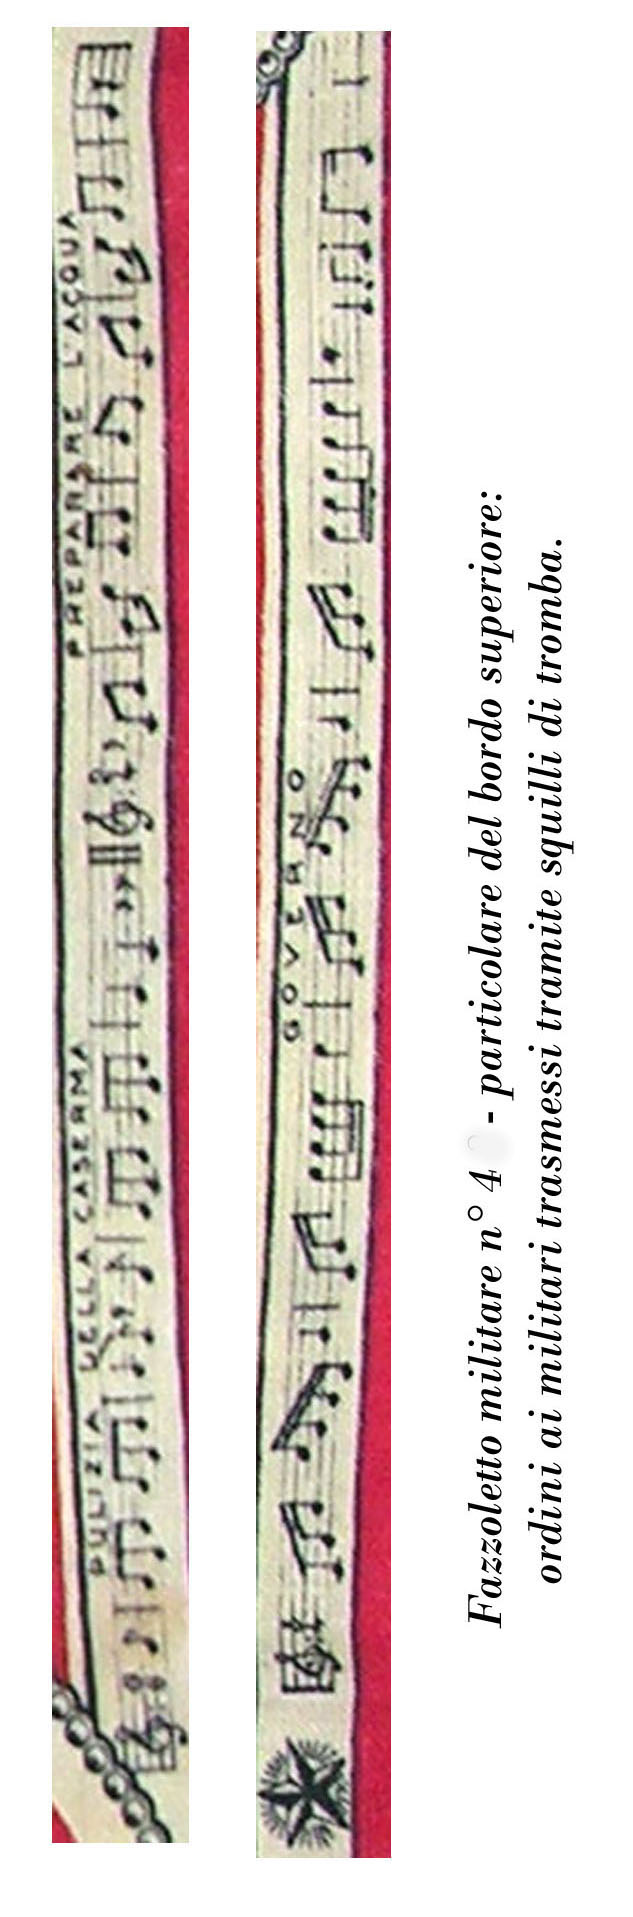
\includegraphics[width=\textwidth]{fazzoletto4_particolare_8.jpg}
	\caption{}
	\label{fig:fazzoletto4_particolare_8}
\end{figure}

\newpage

\begin{figure}[h]
	\centering
		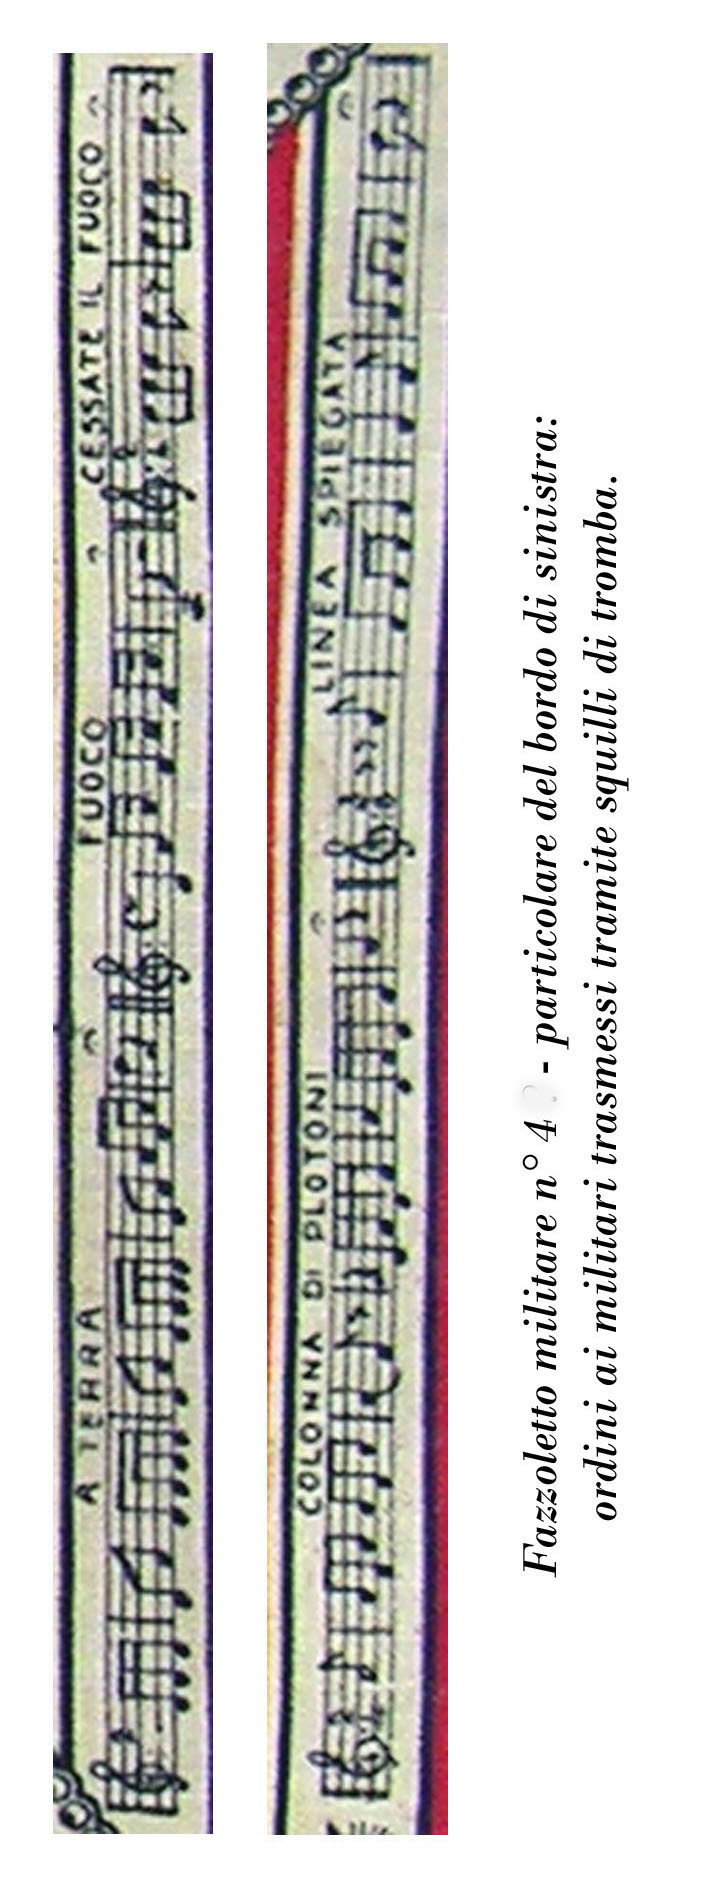
\includegraphics[width=\textwidth]{fazzoletto4_particolare_9.jpg}
	\caption{}
	\label{fig:fazzoletto4_particolare_9}
\end{figure}

\newpage

\begin{figure}[h]
	\centering
		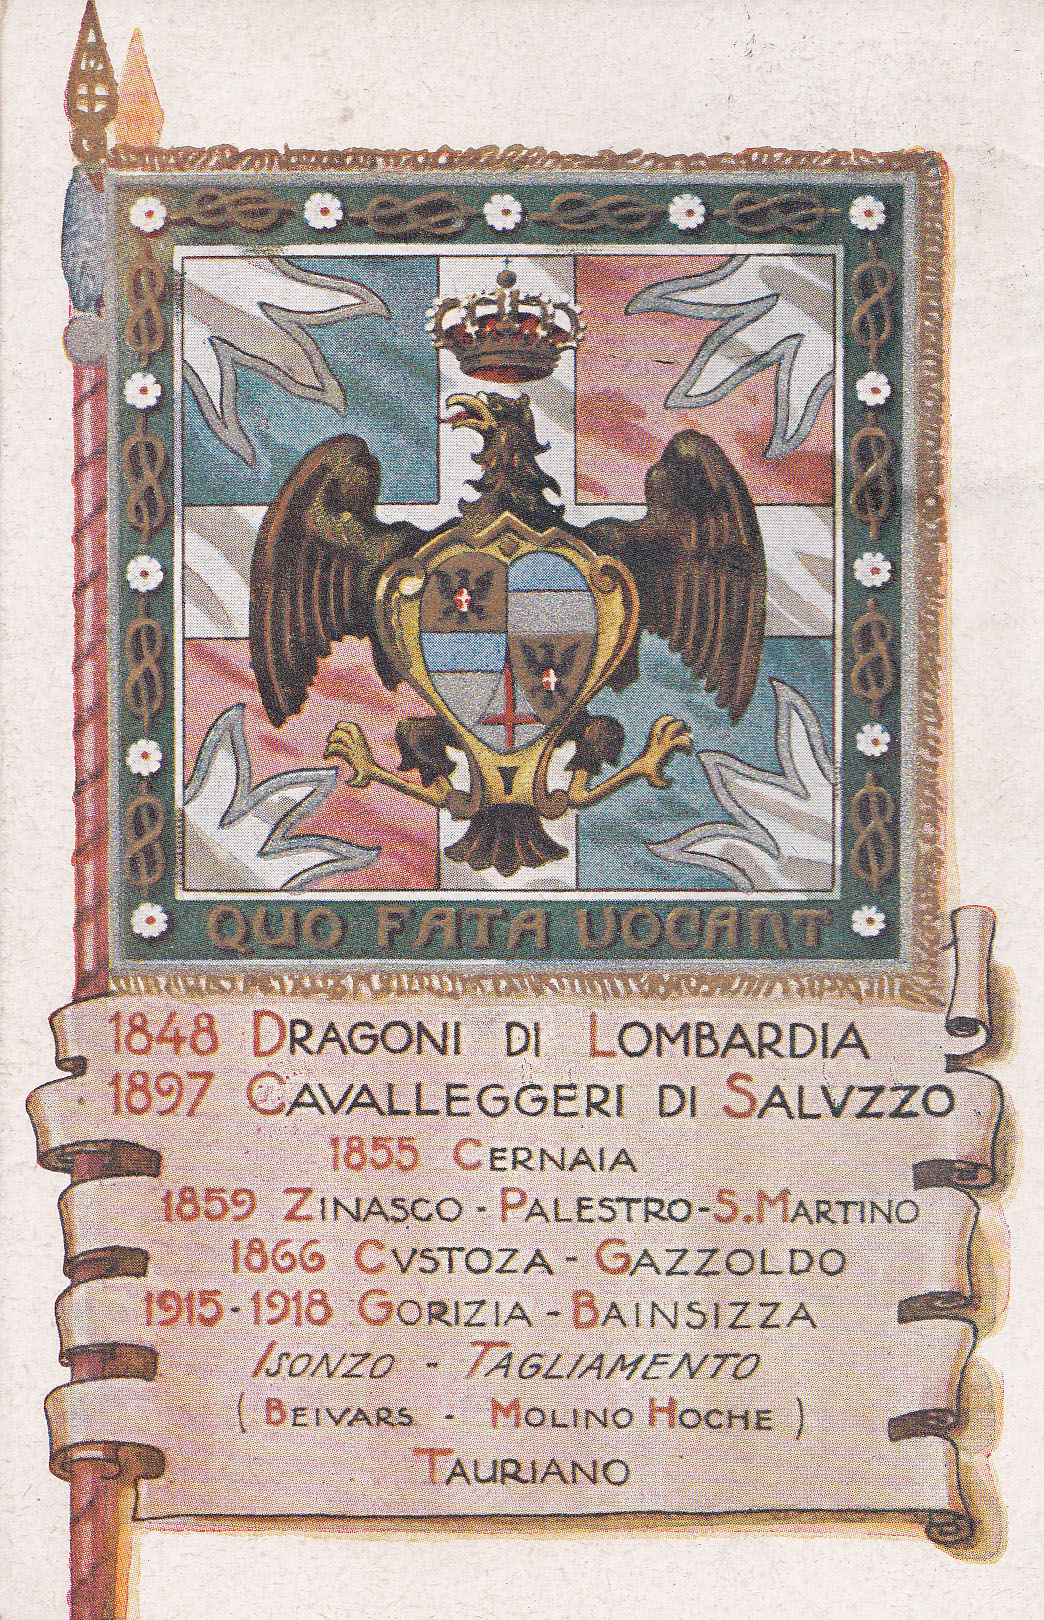
\includegraphics[width=\textwidth]{cartolina_dragoni.jpg}
	\caption{Cartolina emessa per l’Arma della Regia Cavalleria Periodo 1920-1930}
	\label{fig:cartolina_dragoni}
\end{figure}

\newpage

\begin{figure}[h]
	\centering
		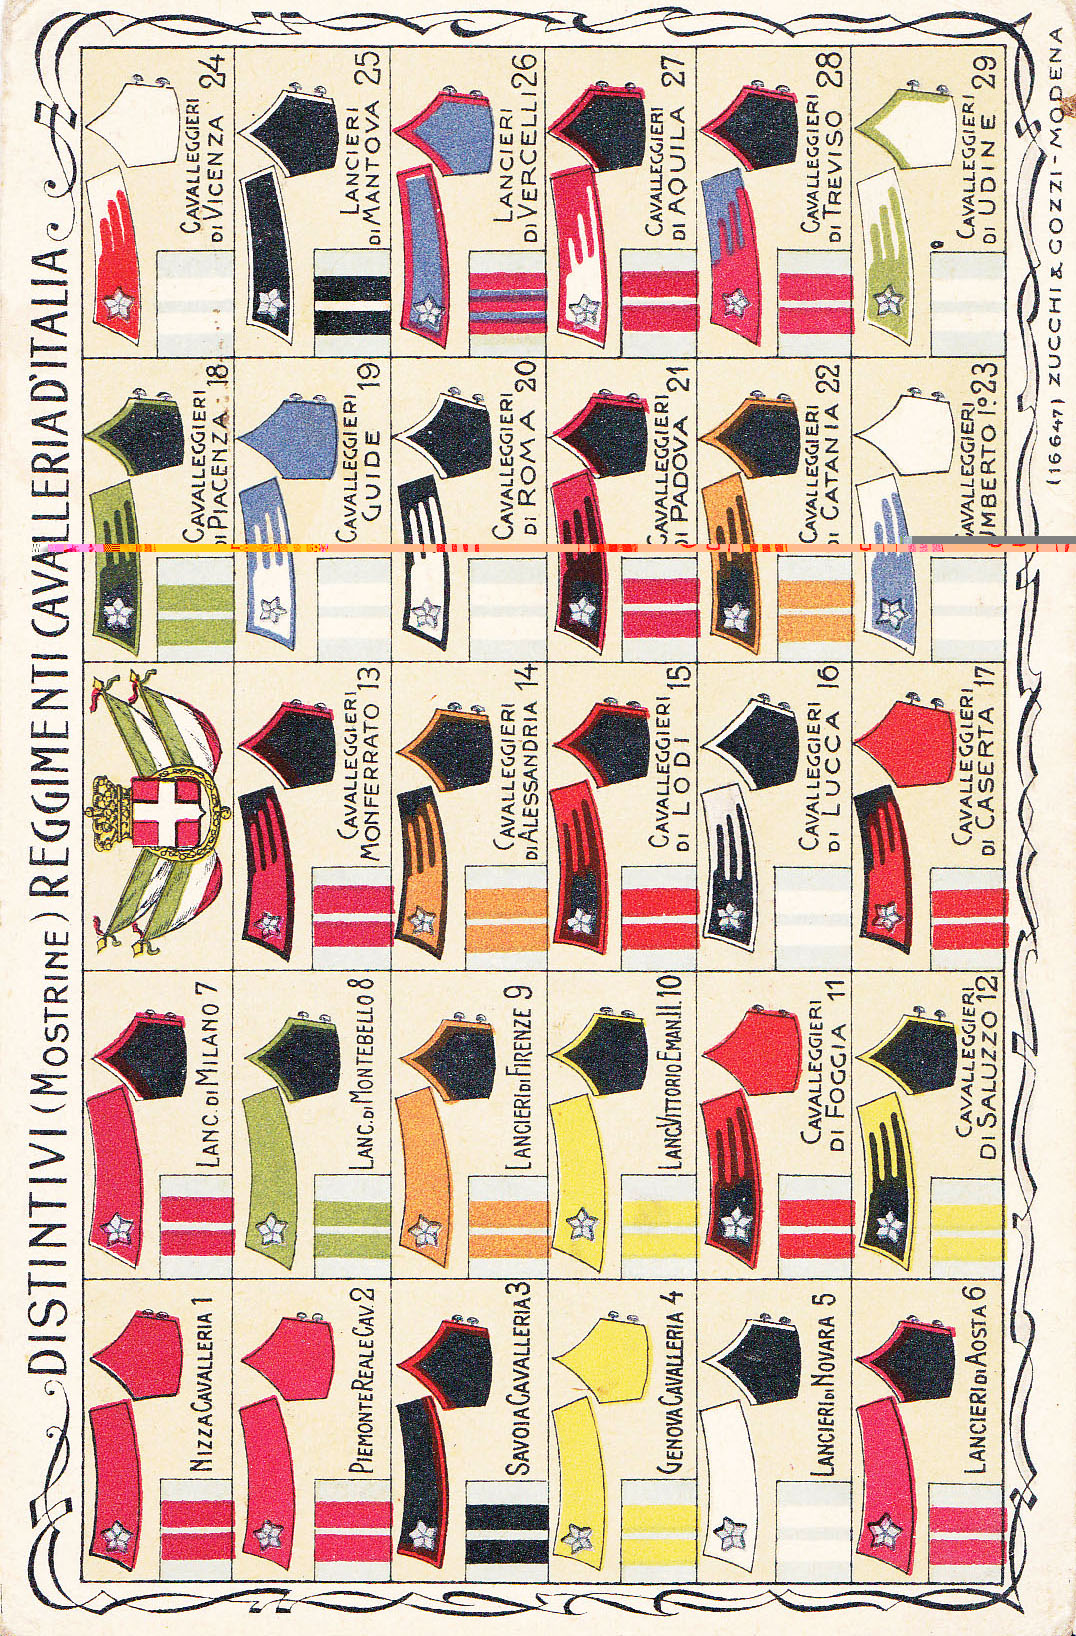
\includegraphics[width=\textwidth]{cartolina_regiacavalleria.jpg}
	\caption{Cartolina emessa per l’Arma della Regia Cavalleria Periodo 1920-1930}
	\label{fig:cartolina_regiacavalleria}
\end{figure}

\newpage

\begin{figure}[h]
	\centering
		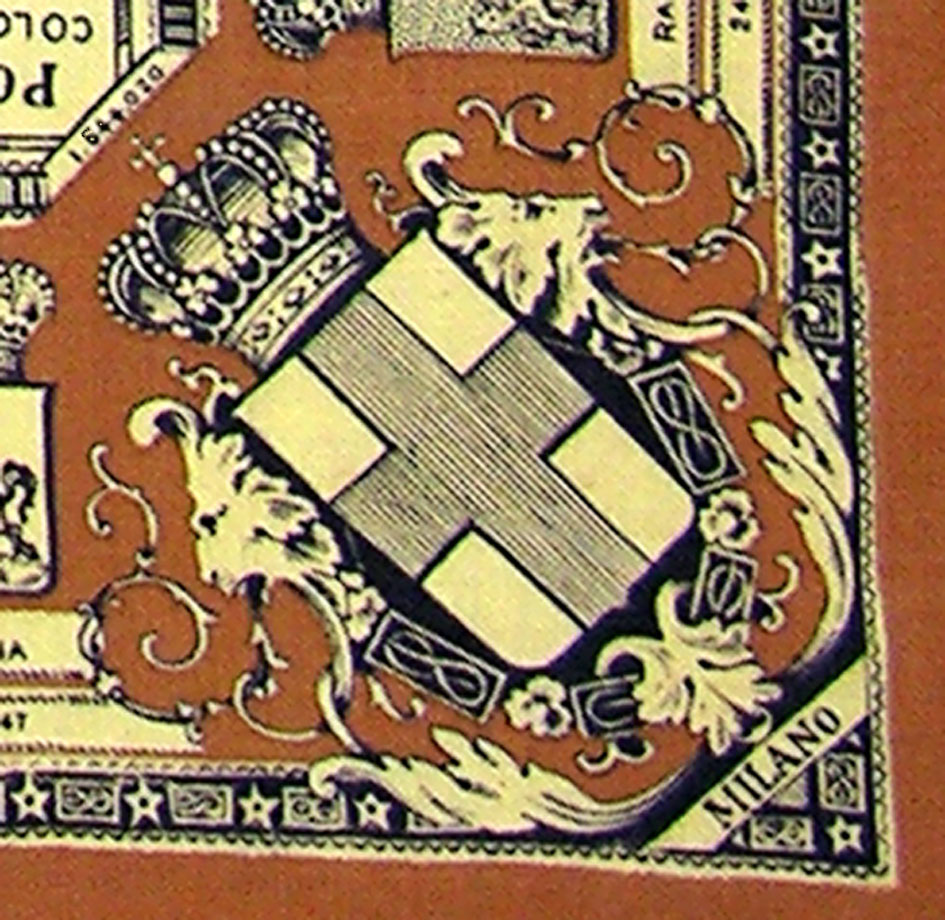
\includegraphics[width=\textwidth]{fazzoletto5_particolare.jpg}
	\caption{Particolare del fazzoletto militare n° 5. Stemma di Milano e numero degli abitanti della Provincia nel 1912}
	\label{fig:fazzoletto5_particolare}
\end{figure}

\newpage

Altre produzioni dell’epoca 1915-18 circa
    I due seguenti fazzoletti vennero prodotti probabilmente durante  il periodo della prima guerra mondiale. Il primo si riferisce all’igiene in ambito domestico. Il secondo è dedicato all’educazione civica. Le frasi riportate sono estrapolate da discorsi che Giuseppe Frua fece alle maestranze in occasione di incontri per ricorrenze o conferimento di attestati.
    
\begin{figure}[h]
	\centering
		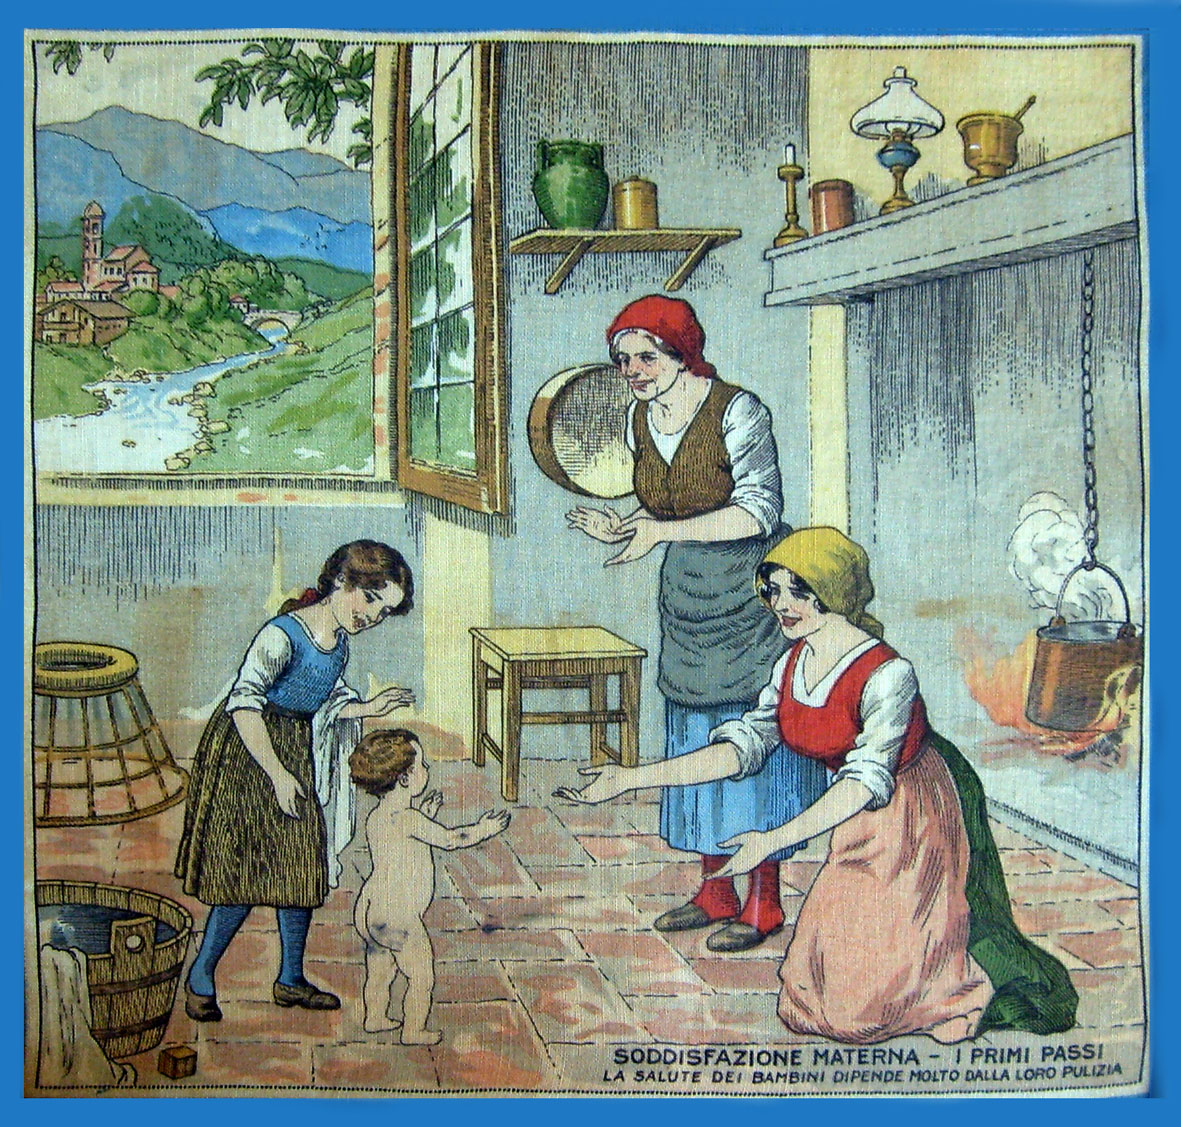
\includegraphics[width=\textwidth]{fazzoletto_educazionefamiliare.jpg}
	\caption{Fazzoletto di educazione famigliare. Dimensioni: 25 x 25 cm}
	\label{fig:fazzoletto_educazionefamiliare}
\end{figure}

\newpage

\begin{figure}[h]
	\centering
		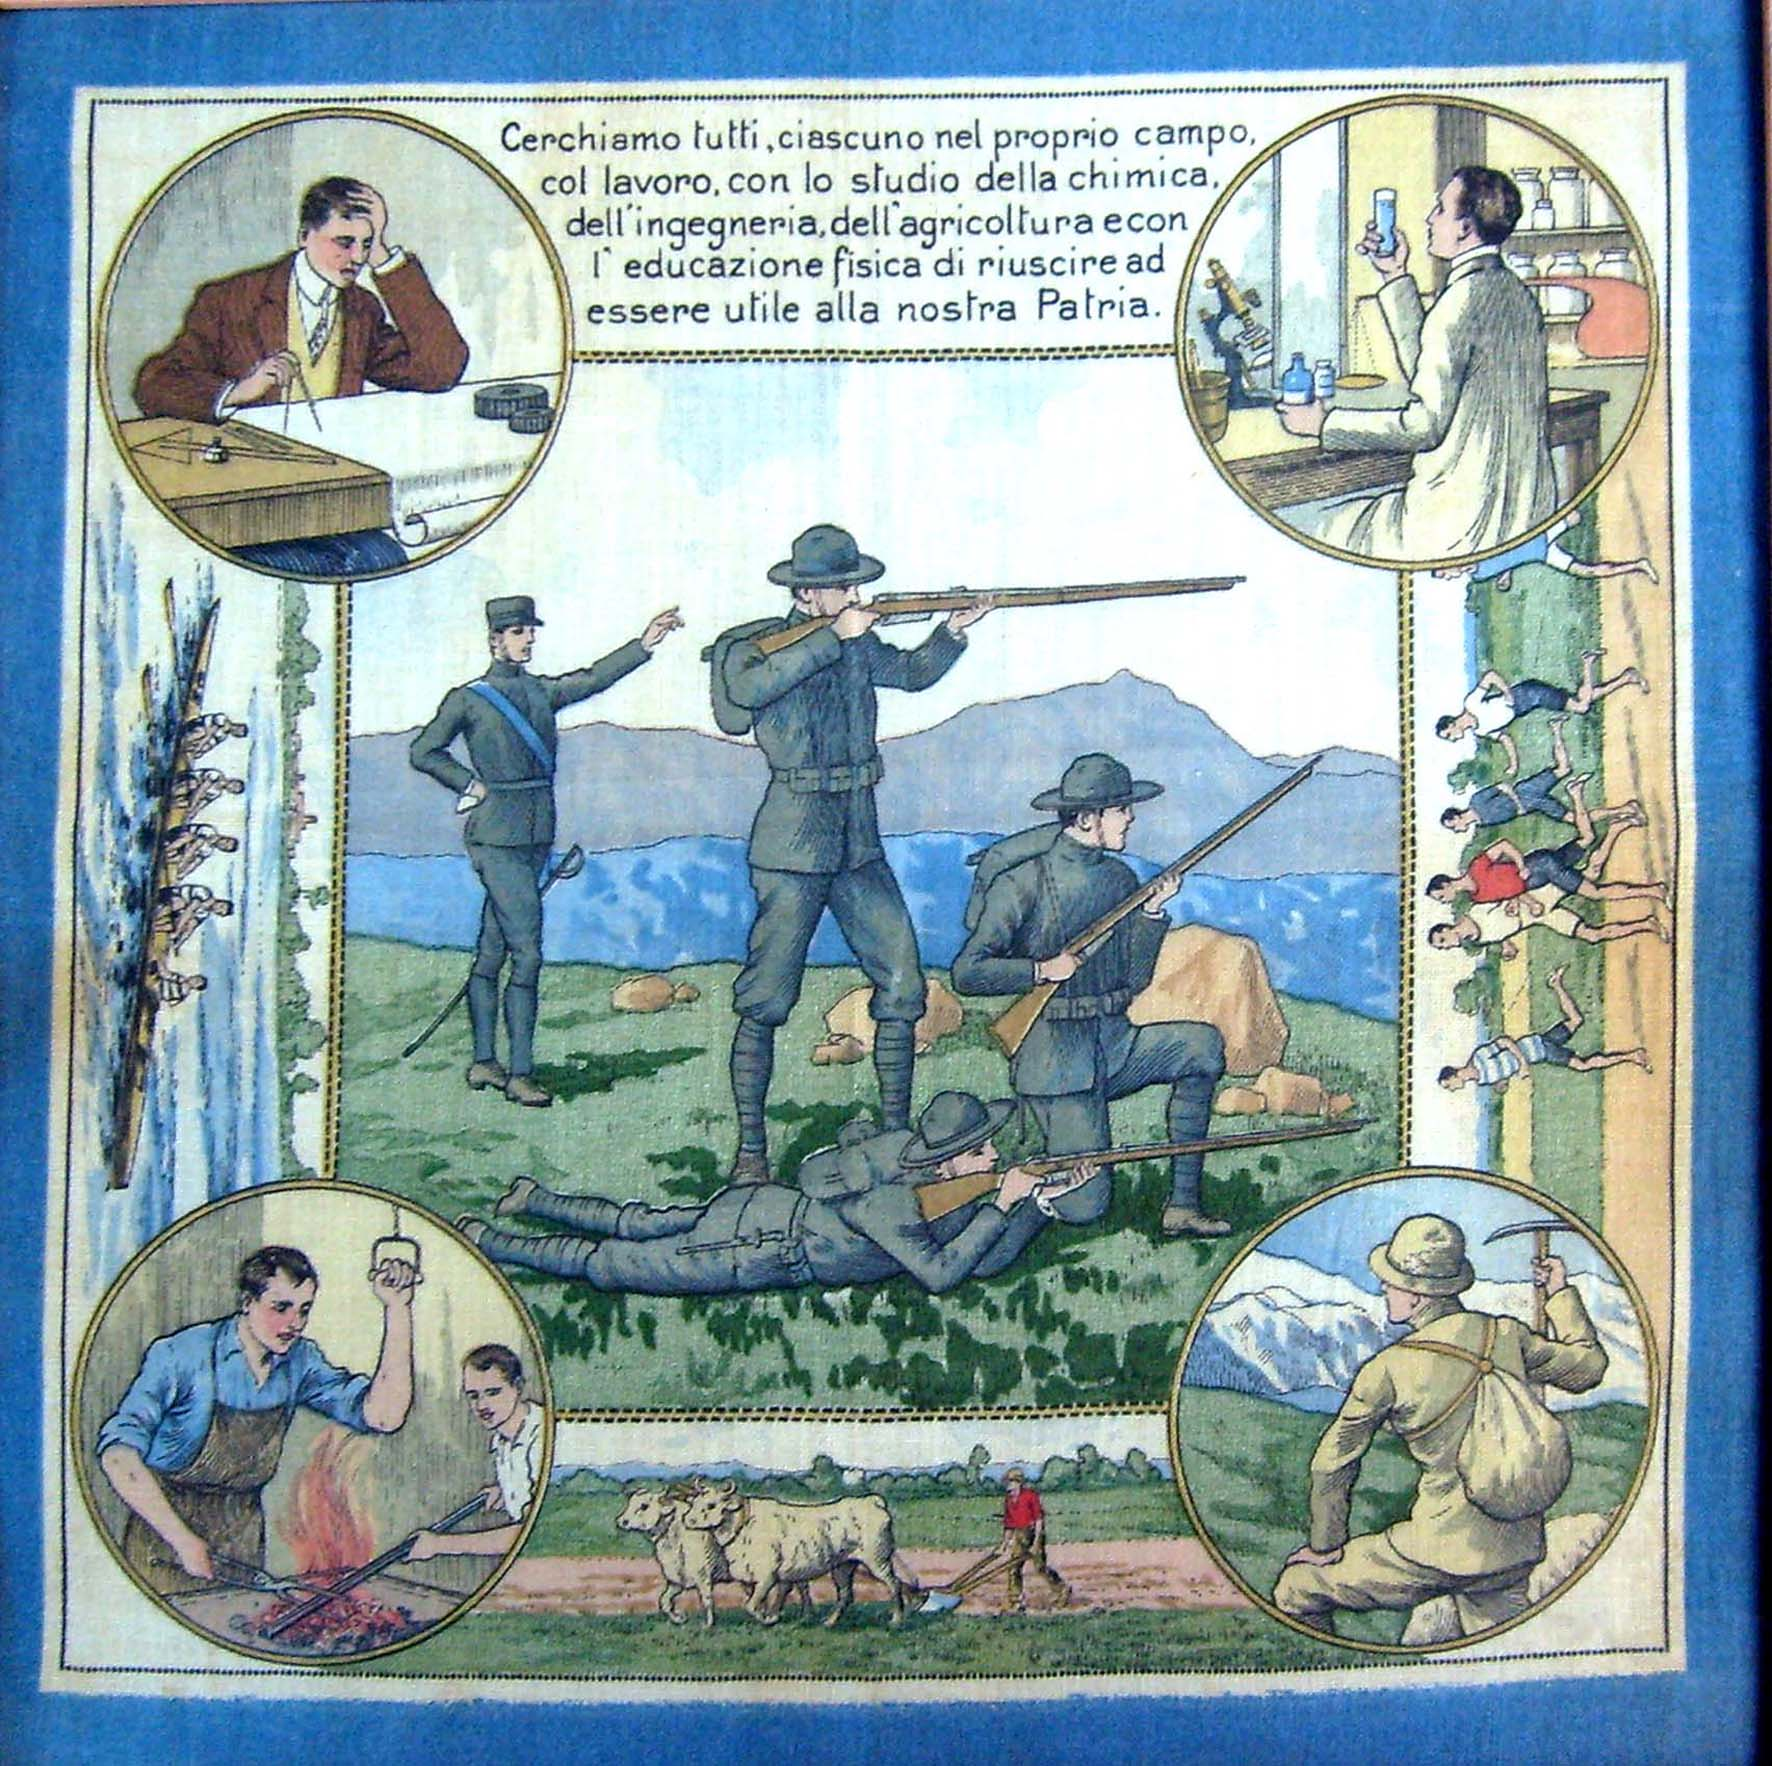
\includegraphics[width=\textwidth]{fazzoletto_educazionecivica.jpg}
	\caption{Fazzoletto di educazione civica  con scritte di Giuseppe Frua. Dimensioni: 27 x 27 cm}
	\label{fig:fazzoletto_educazionecivica}
\end{figure}

\newpage

\begin{figure}[h]
	\centering
		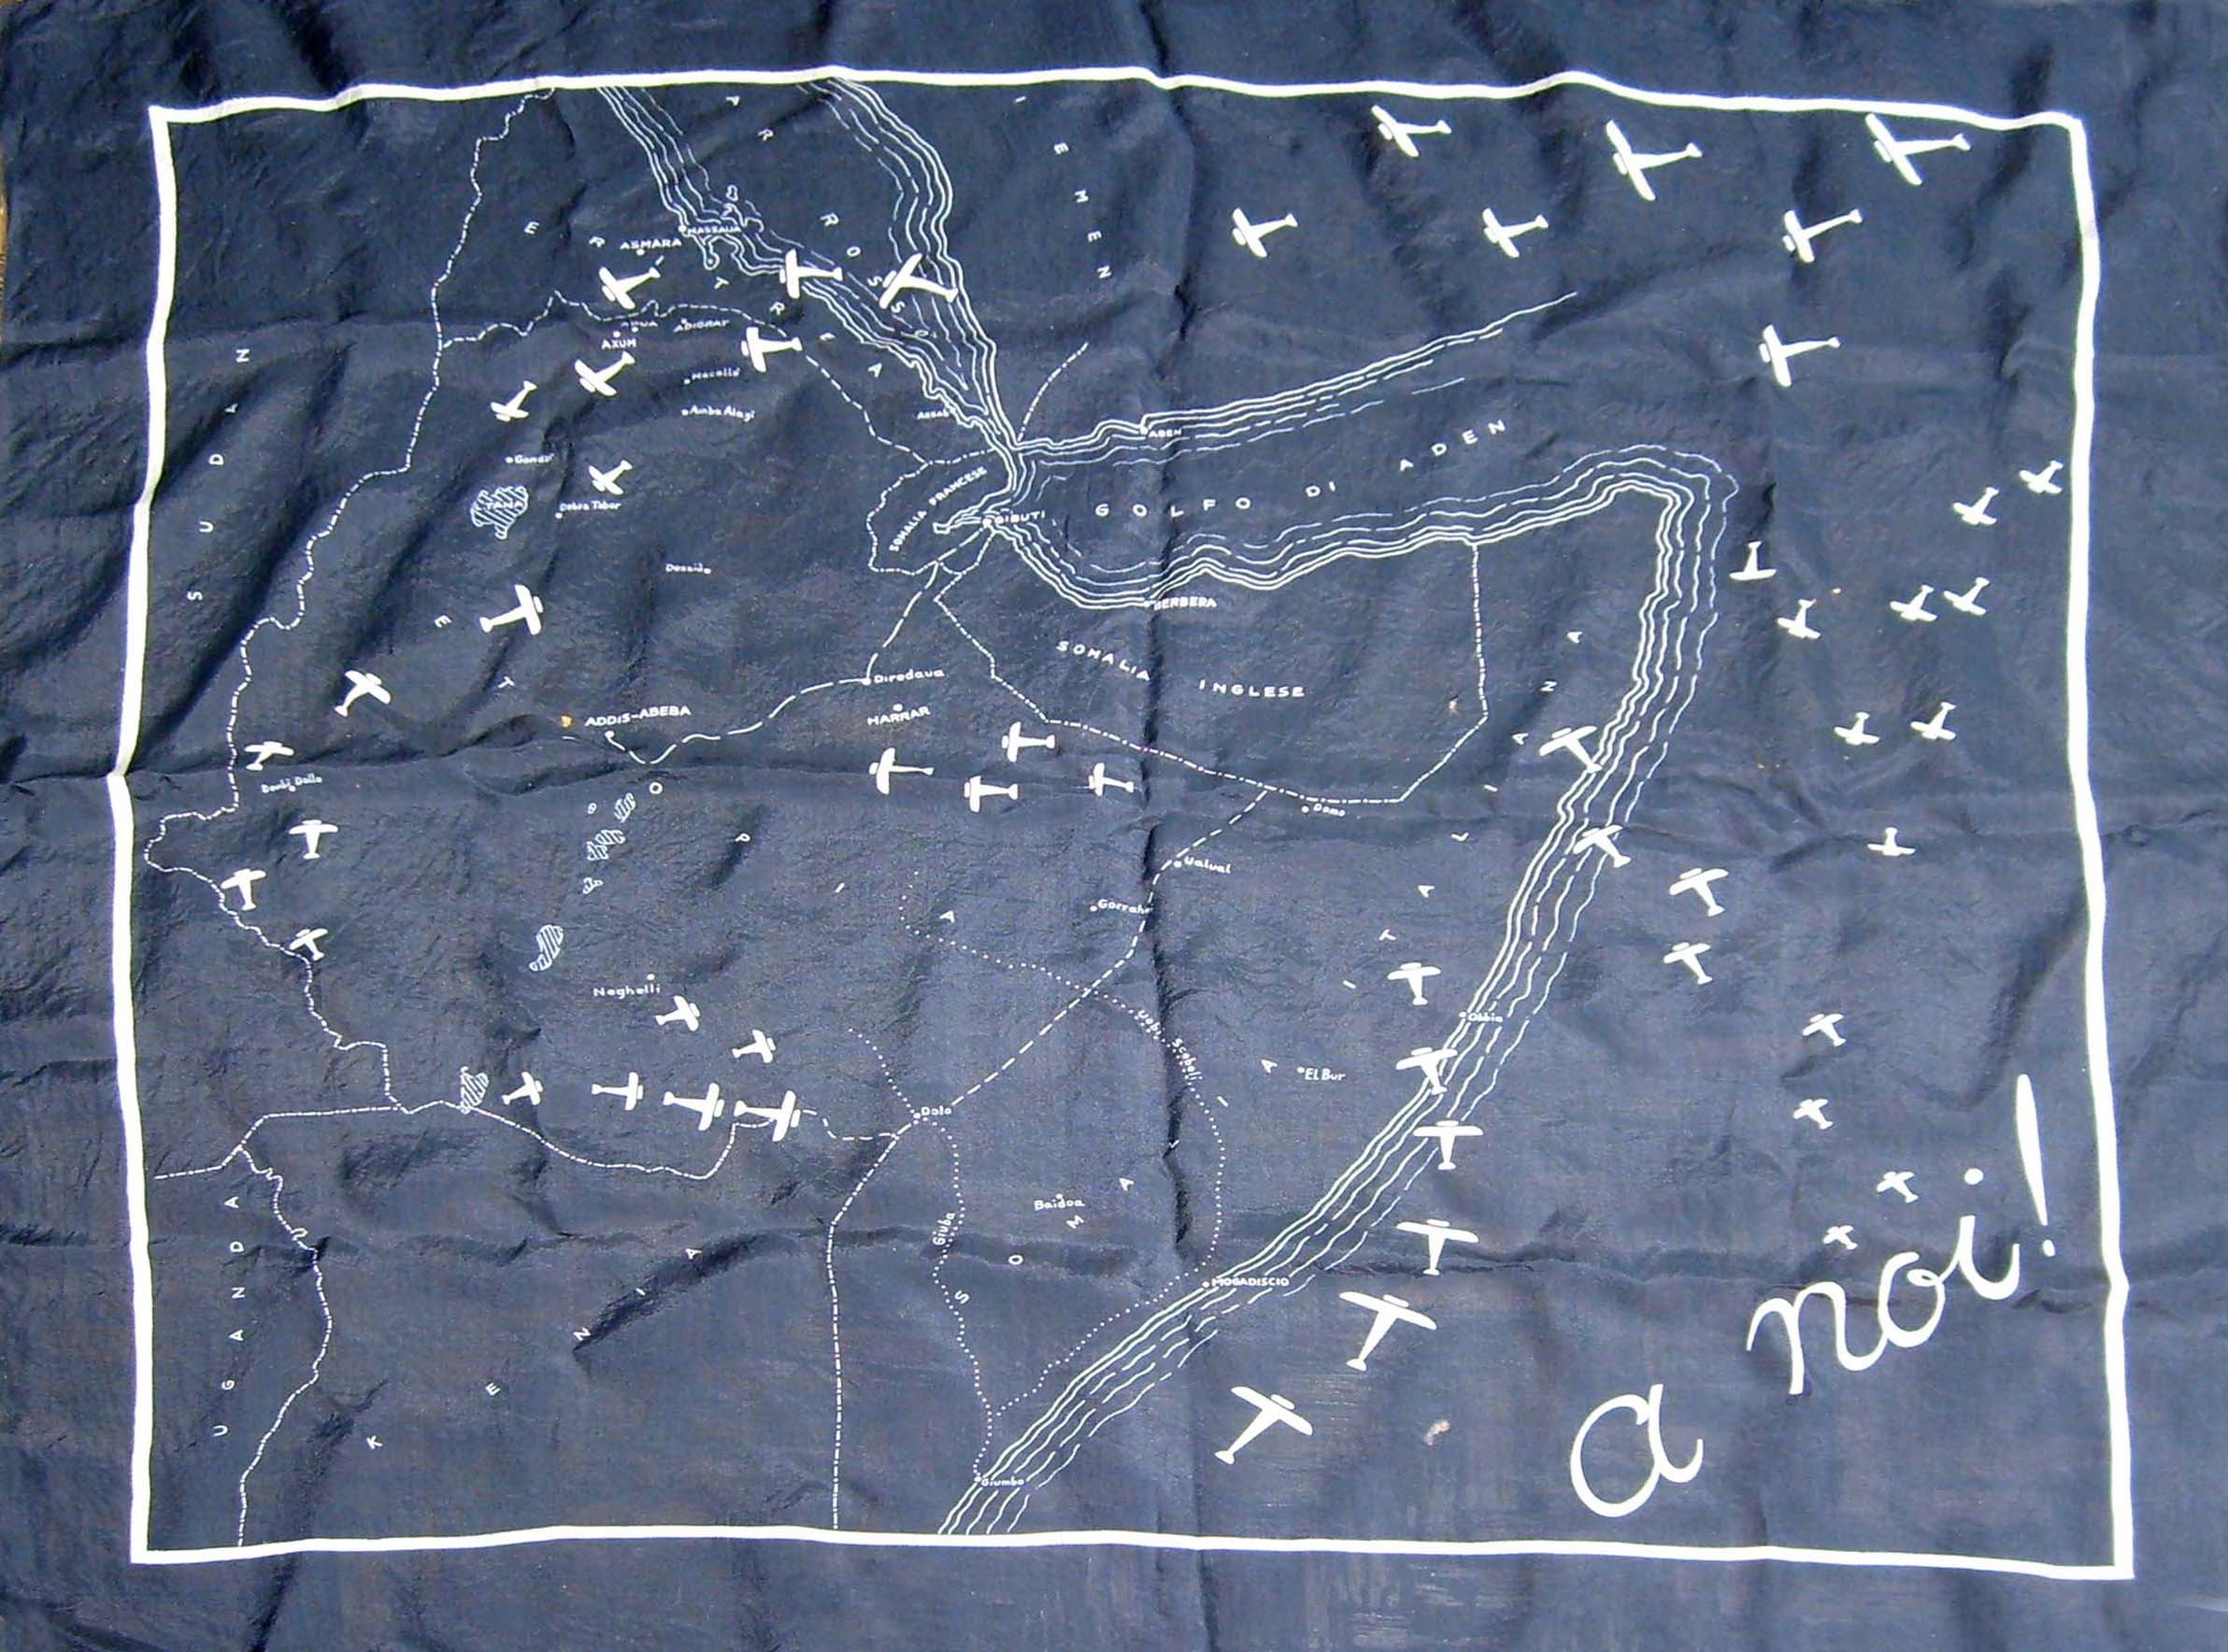
\includegraphics[width=\textwidth]{foulard_etiopia.jpg}
	\caption{Foulard Etiopia del 1935/36. Dimensioni: 78 x 75 cm}
	\label{fig:foulard_etiopia}
\end{figure}

Probabilmente questa produzione fu fatta per il contributo dato dall’Aeronautica militare italiana alla conquista di quel territorio. 

\newpage

\begin{figure}[h]
	\centering
		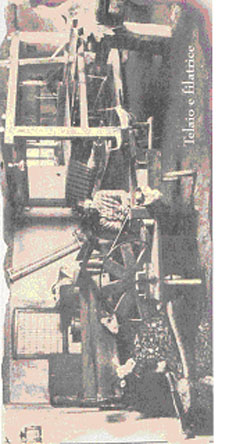
\includegraphics[width=\textwidth]{produzione_casalinga_tessuti.jpg}
	\caption{Produzione casalinga di tessuti fine “800 e inizi “900}
	\label{fig:produzione_casalinga_tessuti}
\end{figure}

\clearpage









































